\documentclass{sbc2023}%

\usepackage{graphicx}
\usepackage[misc,geometry]{ifsym}
\usepackage{fontspec}
\usepackage{fontawesome}
\usepackage{academicons}
\usepackage{color}
\usepackage{xurl}
\usepackage{hyperref}
\usepackage{aas_macros}
\usepackage[bottom]{footmisc}
\usepackage{supertabular}
\usepackage{afterpage}
\usepackage{url}
\usepackage{pifont}
\usepackage{multicol}
\usepackage{multirow}
\usepackage{amsmath}
\usepackage{amssymb}
\usepackage{booktabs}
\usepackage{placeins}

\setcitestyle{square}
\raggedbottom
\setlength{\textfloatsep}{11pt plus 3pt minus 3pt}
\setlength{\dbltextfloatsep}{11pt plus 3pt minus 3pt}

\definecolor{orcidlogo}{rgb}{0.37,0.48,0.13}
\definecolor{unilogo}{rgb}{0.16,0.26,0.58}
\definecolor{maillogo}{rgb}{0.58,0.16,0.26}
\definecolor{darkblue}{rgb}{0.0,0.0,0.0}
\hypersetup{colorlinks,breaklinks,
            linkcolor=darkblue,urlcolor=darkblue,
            anchorcolor=darkblue,citecolor=darkblue}

% Visible DOI formatter for bibliography entries (separate from the JBCS article DOI metadata command).
\newcommand{\bibdoi}[1]{\href{https://doi.org/#1}{doi: #1}}

% Journal metadata are assigned in production by the publisher.
\jid{JBCS}
\jtitle{Journal of the Brazilian Computer Society}
% Article DOI, volume, issue, and publication dates will be assigned by JBCS.
\copyrightstatement{This work is licensed under a Creative Commons Attribution 4.0 International License}

\title[Beyond Random-Split Accuracy]{Beyond Random-Split Accuracy: Distribution Shift, Calibration, and Robustness in Crop Disease Recognition}

% JBCS uses single-blind review: author names and affiliations are shown in the manuscript.
% Author ORCID metadata is not displayed in this submission.
\author[Fadhilah et al.]{
\affil{\textbf{Husni Fadhilah}~\textcolor{blue}{\faEnvelopeO}~~[~\textbf{Department of Informatics, Universitas Diponegoro, Semarang, Indonesia}~|\href{mailto:husnifadhilah62@gmail.com}{~\textbf{\textit{husnifadhilah62@gmail.com}}}~]}

\affil{\textbf{Budi Warsito}~~[~\textbf{Department of Statistics, Faculty of Science and Mathematics, Universitas Diponegoro, Semarang, Central Java, Indonesia}~|\href{mailto:budiwrst@gmail.com}{~\textbf{\textit{budiwrst@gmail.com}}}~]}

\affil{\textbf{Fadhil Elrizanda}~~[~\textbf{School of Electrical Engineering and Informatics, Bandung Institute of Technology, Bandung, Indonesia}~|\href{mailto:23524006@std.stei.itb.ac.id}{~\textbf{\textit{23524006@std.stei.itb.ac.id}}}~]}

\affil{\textbf{Hasna Faridah}~~[~\textbf{Department of Statistics, Institut Teknologi Sepuluh Nopember, Surabaya, Indonesia}~|\href{mailto:hasnafrd01@gmail.com}{~\textbf{\textit{hasnafrd01@gmail.com}}}~]}
}

\begin{document}

\begin{frontmatter}
\maketitle

\begin{mail}
Corresponding author: Husni Fadhilah, Universitas Diponegoro, Semarang, Indonesia. E-mail: \href{mailto:husnifadhilah62@gmail.com}{husnifadhilah62@gmail.com}.
\end{mail}



\begin{abstract}
\textbf{Abstract.~}
\noindent Reliable image-based crop disease recognition requires models to work beyond curated benchmark images, since real-world backgrounds, illumination, and image artifacts may differ from training conditions. Yet random image splits can yield very high classification scores without establishing how a model behaves when image conditions change. This study evaluated ImageNet-pretrained classifiers using PlantVillage as the in-domain benchmark and PlantDoc and Cassava as external distribution-shift datasets. The exact-duplicate-exclusion reference achieved macro-F1 0.996191 on 5,426 unaffected test images, while a stricter full group-deduplication sensitivity analysis, combining exact hashes and near-pHash connected components, achieved macro-F1 0.996661 on 5,316 test images. The conventional fixed-split benchmark achieved macro-F1 0.997141 and balanced accuracy 0.996853 on 5,431 test images. Across three independently trained seeds, external OOD AUROC averaged 0.954748 (standard deviation, SD, 0.020819) for PlantDoc and 0.981930 (SD 0.017199) for Cassava. Validation-fitted temperature scaling gave test ECE 0.000876. A GPU inference benchmark on a separate Tesla T4 runtime measured 0.6602 to 2.9255 ms per image across the compared backbones, without treating that runtime as the historical training hardware. Blur-aware training increased motion-blur macro-F1 from 0.4287 to 0.9013 but reduced performance under square occlusion and red-channel color shift. The principal contribution is a protocol-separated empirical reliability audit that exposes where near-ceiling benchmark performance ceases to justify stronger claims, rather than a new classifier or OOD algorithm. Together, these findings support reporting deduplication sensitivity, calibration, external-shift variability, computational measurements, and perturbation-specific robustness as distinct quantities.
\end{abstract}

\begin{keywords}
EfficientNet, out-of-distribution detection, PlantDoc, PlantVillage, selective prediction, temperature scaling.
\end{keywords}

\end{frontmatter}

\section{Introduction}\label{sec:intro}
Image-based crop disease recognition has reached very high accuracy on benchmark datasets, but the meaning of that accuracy depends strongly on how the images were collected and split. The PlantVillage release provided more than 50,000 expertly curated images of healthy and diseased crop leaves and was intended to support machine-learning research on plant-health diagnosis \cite{r01}. PlantDoc was later introduced specifically because sufficiently large non-laboratory datasets were scarce, and its authors assembled 2,598 annotated image data points from internet-scraped imagery \cite{r02}. These two resources therefore represent substantially different acquisition settings. The Cassava benchmark adds a separate, five-class cassava disease setting with highly variable field backgrounds and a distinct plant-species and disease-label space \cite{r03}. As a result, the three collections provide complementary but confounded scenarios for studying model confidence under distribution shift.

Recent work has made the field-versus-benchmark distinction more explicit. Mahapatra et al. evaluated both intra-dataset and cross-dataset plant-disease classification and reported substantially lower cross-dataset accuracy than their best intra-dataset result \cite{r39}. Zhang and Liu focused on field-acquired PlantDoc images and designed a multi-scale Vision Mamba model for complex backgrounds and fine-grained lesion patterns \cite{r14}. These studies support treating cross-dataset behavior as a separate question from performance on a random split of one collection.

A second issue is the reliability of predictive confidence. Guo et al. showed that modern neural networks can be poorly calibrated and found single-parameter temperature scaling to be effective on multiple benchmarks \cite{r04}. Liu et al. proposed an energy score for OOD detection because softmax confidence can remain high on unfamiliar samples \cite{r05}. Li et al. benchmarked ten OOD methods with AUROC, FPR@95, and AUPR, showing the value of evaluating more than one OOD metric \cite{r42}. These reliability measures complement accuracy rather than replace it.

Robustness under image perturbation is another distinct concern. Enkvetchakul and Surinta found that specific combinations of rotation, shift, and zoom augmentation improved plant-leaf recognition performance in their experiments \cite{r06}. Park et al. combined test-time training, Mixup, and entropy-based sample ordering to improve corruption robustness on the CIFAR10-C benchmark \cite{r11}. Such findings motivate testing augmentation and robustness under explicitly defined perturbations instead of assuming that an augmentation policy improves every type of shift.

The research gap is not an absence of classifiers or individual reliability metrics. Rather, existing benchmark reports often leave the evidential relationships among image-level leakage, probability calibration, external semantic and visual shifts, stochastic variation, and corruption-specific training unclear. A very high fixed-split score alone cannot establish whether the same checkpoint is calibrated under shift or whether robustness gains transfer between perturbations. This study addresses that gap through a structured empirical audit rather than a novel network architecture. Its contributions are: (i) a leakage-aware comparison of the original PlantVillage split and duplicate-exclusion sensitivity retraining, (ii) a protocol-traced assessment of calibration, selective prediction, and two heterogeneous OOD datasets, (iii) an explicit separation of full fine-tuning from frozen-feature and corruption-aware experiments, and (iv) a matched perturbation-specific comparison showing both gains and regressions. PlantDoc and Cassava are not treated as matched-label disease test sets. The purpose is to determine which reliability claims are supported, which are protocol-conditional, and which require prospective field validation.

\section{Related Work}\label{sec:related}
\subsection{Dataset realism, field imagery, and cross-dataset evaluation}
PlantVillage remains a widely used leaf-image benchmark for crop-disease classification \cite{r01}. PlantDoc was designed to reduce the lack of non-laboratory imagery and includes manually annotated images collected from the internet \cite{r02}. The Cassava benchmark used by Zhong et al. is strongly imbalanced and includes background variability that can interfere with conventional convolutional feature extraction \cite{r03}. These differences in acquisition conditions are important because an external dataset can introduce both semantic and visual distribution changes.

Singh and Gahlawat reviewed how PlantVillage and PlantDoc are used for machine-learning-based disease prediction and emphasized the role of dataset composition in model training and evaluation \cite{r16}. Saini et al. used PlantDoc for multi-crop disease detection and combined classification with object localization in diseased regions \cite{r30}. Sarada presented a comparative analysis of AI techniques specifically on the PlantDoc dataset, illustrating the continued use of PlantDoc as an evaluation resource for field-oriented imagery \cite{r35}.

Field datasets outside PlantDoc provide another view of realism. Anami et al. used field images to classify 12 categories of biotic and abiotic paddy stresses with a pretrained VGG-16-based framework \cite{r40}. Fenu and Malloci introduced DiaMOS Plant as a dataset aimed at diagnosis and monitoring rather than only static benchmark classification \cite{r41}. Together, these datasets motivate separating controlled-image performance from claims about field deployment.

\subsection{Architectures, transfer learning, and computational design}
Architecture design in plant-disease recognition ranges from conventional CNNs to recent lightweight and state-space models. Roopa et al. explicitly framed their PlantVillage study as a generalized cross-crop deep-learning approach \cite{r08}. Xu and Li combined feature recalibration with an improved residual network and reported the FRseNet architecture for crop pest and disease recognition \cite{r10}. The existence of multiple high-performing architectures makes protocol consistency especially important when comparing models.

Transfer learning is common when agricultural datasets are limited. Setiawan et al. evaluated InceptionV3 and Xception with transfer learning and augmentation for rice disease recognition, with Xception giving the strongest result in their reported experiment \cite{r17}. Nidhi Singh evaluated VGG16, ResNet50, and InceptionV3 with transfer learning and also discussed synthetic data generation using GANs for plant-disease recognition \cite{r22}. Ali et al. trained a compact CNN on the 38-condition PlantVillage benchmark and reported 92.3\% validation accuracy after ten epochs \cite{r23}.

Computational efficiency has also been studied directly. Kumar and Singh investigated the computational response and performance of deep convolutional networks for plant-disease classification on leaf data \cite{r24}. Verma et al. proposed DynLeafNet as a lightweight dynamic residual architecture and paired it with explainable-AI analysis \cite{r26}. Nagrath et al. compared CNN, DenseNet transfer-learning variants, an ensemble, and a DenseNet201-LSTM hybrid for medicinal-plant recognition \cite{r29}.

The broader applied literature includes both implementation-focused and survey-style studies. Akila et al. reported a deep-learning plant-disease detection system in a recent application study \cite{r31}. Simhadri discussed machine-learning and deep-learning approaches including CNNs, support-vector machines, and k-nearest neighbors for plant-disease detection \cite{r32}. Zheng et al. reviewed crop-disease recognition based on spectral and RGB imagery and covered recent paradigms including state-space models and generative AI \cite{r38}. These studies show that architecture choice is only one part of a larger evaluation problem that also includes data quality and deployment conditions.

\subsection{Augmentation, imbalance, and generalization}
Data augmentation is frequently used to reduce overfitting and improve representation diversity. Enkvetchakul and Surinta reported that rotation, shift, and zoom were useful in their MobileNetV2 and NASNetMobile plant-leaf experiments \cite{r06}. Min et al. proposed a dedicated data-augmentation method for plant-leaf disease recognition and evaluated augmentation as part of the recognition pipeline \cite{r09}. Lee and Lee evaluated geometric and color-space augmentation on a 24-class crop-disease dataset and reported F1 scores above 98\% in their experiments \cite{r27}.

Several studies focus on augmentation when datasets are small or imbalanced. Huang investigated combined augmentation as a way to mitigate overfitting in plant-disease recognition \cite{r28}. Fawaiq et al. used augmentation together with VGG16, NASNetMobile, and Xception for rice-leaf disease detection and reported the best test accuracy with Xception \cite{r33}. Xu et al. proposed style-consistent image translation so that variations learned from one class can be transferred to another while preserving unrelated image content \cite{r34}.

Long-tailed and imbalance-aware settings require additional care. Zhang et al. studied long-tailed recognition specifically for food-crop disease images \cite{r13}. Zhang proposed an improved CNN with augmentation and regularization for rice leaf pest and disease recognition and reported a large gain over the baseline model in that experiment \cite{r37}. These results reinforce the need to describe the augmentation and imbalance protocol explicitly rather than treating all training recipes as equivalent.

\subsection{Calibration, uncertainty, OOD detection, and corruption robustness}
Calibration asks whether reported probabilities correspond to empirical correctness frequencies. Guo et al. found that contemporary neural networks can be miscalibrated and identified temperature scaling as an effective post-hoc method on several datasets \cite{r04}. Balanya et al. generalized temperature scaling through adaptive temperature functions and proposed an entropy-based variant designed to remain useful when calibration data are limited \cite{r21}. Bae and Kim proposed accuracy-informed label smoothing and logit scaling and reported calibration improvements, including under distribution shifts augmented during training \cite{r20}.

Uncertainty can also be represented through prediction intervals or selective procedures. Parra and S\'aez proposed deep-learning prediction intervals based on selective joint supervision and evaluated them on nonlinear dynamic systems \cite{r25}. Although their application is not crop classification, the work provides a methodological example of explicitly modeling predictive uncertainty rather than relying only on point predictions.

OOD detection addresses a different question: whether an input should be treated as unfamiliar relative to the training distribution. Liu et al. showed that energy scores can separate in- and out-of-distribution samples better than softmax confidence in their benchmark settings \cite{r05}. Li et al. compared ten OOD methods on remote-sensing scene datasets and evaluated them with AUROC, FPR@95, and AUPR \cite{r42}. The present study follows the same principle of treating OOD ranking and in-domain classification as separate outcomes.

Robustness to image corruption is similarly distinct from ordinary test accuracy. Mitra et al. studied the interaction among post-hoc pruning, uncertainty calibration, and natural corruption robustness in image-classification CNNs \cite{r07}. Park et al. improved corruption robustness through test-time training combined with Mixup and entropy-based sample ordering \cite{r11}. These works motivate the paired corruption experiments reported here.

\subsection{Explainability and application-oriented systems}
Some recent plant-disease systems combine classification with explainability or user-facing software. Kumar and Priyamvada used pretrained InceptionV3 and MobileNetV2 models in a Flask-based web application that accepts leaf images, returns disease predictions, and retrieves information from a disease knowledge base \cite{r12}. Sravan and Rajagopalan described a full-stack application that combined CNN-based disease classification with severity assessment \cite{r15}. Shanukumar Singh et al. evaluated deep-learning disease detection from leaf images and compared results before and after augmentation and preprocessing \cite{r18}.

Application papers also explore direct decision-support interfaces. Patange et al. presented PlantDocBot as an AI-based system for early crop-disease detection and described it as a scalable diagnostic interface \cite{r19}. Joseph and Pawar devoted a book chapter to explainable artificial intelligence for plant-disease diagnosis \cite{r36}. These systems are relevant to deployment, but user-facing software does not itself establish robustness under unseen acquisition conditions.
\subsection{Critical synthesis and evidence gap}
The surveyed literature provides strong individual contributions to plant-image classification, augmentation, calibration, OOD scoring, and robust evaluation. However, these results do not define a common notion of reliability. Calibration evaluates agreement between predicted confidence and empirical correctness on labeled data. Predictive uncertainty describes the ambiguity of individual predictions, while selective prediction evaluates performance after abstaining on low-confidence inputs. OOD detection instead ranks inputs by unfamiliarity relative to a specified reference distribution. Corruption robustness measures changes in task performance under defined image perturbations. Consequently, an OOD AUROC should not be interpreted as field classification accuracy, and a low in-domain ECE does not establish calibration in a different label space.

The unresolved question addressed here is empirical and methodological in its reporting rather than algorithmic: how conclusions change when leakage, checkpoint provenance, score calibration, external dataset heterogeneity, and corruption protocols are checked side by side. Combining these diagnostics alone is not claimed as a new method. The additional evidence comes from documenting apparent performance contradictions, including an exact-duplicate sensitivity retraining and a matched corruption study in which gains under one perturbation accompany degradation under others.

\section{Materials and Methods}\label{sec:methods}
\subsection{Study design, datasets, and split}
All evaluations were retrospective and computational. The conventional fixed-split EfficientNet-B0 full fine-tuning run provides the main benchmark checkpoint for in-domain recognition, validation-fitted calibration, and PlantDoc/Cassava confidence-based OOD scoring. A separate leakage-aware retraining excludes exact MD5 cross-split groups and produces a distinct test-set estimate. Frozen-feature architecture and data-fraction comparisons, seed-variation runs, and the independently trained corruption-aware models are distinct protocols and must not be represented as tests of one shared checkpoint. The workflow in Fig.~\ref{fig:workflow} and Table~\ref{tab:protocol_map} distinguish the linked and independently trained branches. Validation data selected checkpoints and fitted temperature. The held-out test split was evaluated only after those choices. External images were assessed without mapped disease-class accuracy.


PlantVillage served as the in-domain reference. The PlantVillage repository provides the in-domain leaf-image reference used in this study \cite{r01}. The verified color mirror used here contained 54,305 files across 38 classes. A two-stage stratified random split used seed 42: first, 80\% of the images were assigned to training and 20\% to a temporary holdout, and then that holdout was divided equally by a second stratified split using the same seed. The resulting training, validation, and test subsets contained 43,444, 5,430, and 5,431 images, respectively, or approximately 80\%, 10\%, and 10\%. Stratification used the 38 disease-class labels and was not group-disjoint by acquisition identity. PlantDoc was used as an external field-style dataset. The original PlantDoc publication reports 2,598 image data points spanning 13 plant species and up to 17 disease classes \cite{r02}. The Kaggle mirror used in this study contained only a \texttt{test/} directory, with 252 images arranged in 27 folders. Those 252 images were used only for external diagnostics.

The Cassava mirror contained 21,397 images across five classes. It originated from the Makerere University AI Lab cassava competition. A peer-reviewed cassava study using the same 21,397-image benchmark documents the five-class, imbalanced cassava disease setting \cite{r03}. Cassava additionally represents a distinct five-class, field-oriented cassava-leaf diagnosis setting with a highly imbalanced label distribution. Its plant species and disease taxonomy differ from PlantVillage as well as from the selected PlantDoc mirror. Including it therefore tests the response of PlantVillage-trained confidence scores to a second heterogeneous external collection rather than providing a second matched-label classification benchmark. Because PlantVillage, PlantDoc, and Cassava use different class definitions and acquisition conditions, disease-class accuracy was not compared across datasets.

\begin{table*}[!t]
\centering
\caption{Relationships among the principal experimental protocols. Only outcomes from the same row and checkpoint should be treated as paired or directly comparable.}
\label{tab:protocol_map}
\small
\begin{tabular}{p{0.21\textwidth}p{0.35\textwidth}p{0.34\textwidth}}
\toprule
Protocol & Model and data & Permitted interpretation \\
\midrule
Conventional benchmark & Fully fine-tuned EfficientNet-B0, seed 42, 43,444/5,430/5,431 & Original fixed-split in-domain benchmark \\
Primary leakage-controlled reference & Independently retrained EfficientNet-B0 with 14 cross-split MD5 duplicates excluded & Conservative leakage-controlled estimate on 5,426 unaffected test images \\
Extended deduplication sensitivity & Independently retrained EfficientNet-B0 after excluding 159 connected cross-split components formed from exact hashes and near-pHash links & Broader descriptive sensitivity estimate on 5,316 test images. It was not directly pooled with the primary reference \\
Seed confirmation & Independently trained EfficientNet-B0 runs with seeds 7, 42, 123 on one fixed partition & Sensitivity to initialization and training randomness, not to different data splits \\
Frozen-feature benchmarks & Separately trained linear heads on frozen features, common test items & Within-protocol architecture and sample-fraction comparisons \\
Corruption protocols & Primary basic, separately trained corruption-aware, and a matched basic/blur-aware pair & Matched comparisons only within the specified pair and perturbation settings \\
\bottomrule
\end{tabular}
\end{table*}


\subsection{Exploratory data analysis}
The dataset EDA was performed before model training using the distribution report and duplicate audit. For PlantVillage, all 38 class directories were enumerated and 50 images per class were sampled for image-level profiling. The profile recorded class count, median width and height, channel-wise mean intensity, and median edge density. PlantVillage contained 54,305 images. Class counts ranged from 152 (Potato healthy) to 5,507 (Orange huanglongbing), giving an observed class-imbalance ratio of 36.23. The sampled PlantVillage images had a median spatial size of 256$\times$256 pixels across the recorded classes. The corresponding dataset inventories contained 252 PlantDoc images across 27 classes and 21,397 Cassava images across 5 classes. These counts refer to the dataset copies used in the experiments.

The EDA also characterized acquisition context and label availability. PlantVillage images were predominantly laboratory-style, whereas PlantDoc and Cassava represented field or field-oriented imagery in the dataset metadata. None of the three primary mirrors supplied the farm, cultivar, session, device, or severity metadata required for group-aware or severity-stratified analysis. The duplicate audit covered all 54,305 images under the PlantVillage \texttt{color/} directory. It identified 21 MD5 duplicate groups involving 42 images, 22 exact perceptual-hash groups involving 44 images, and 383 perceptual-hash pairs with Hamming distance at most 4. Reconstructing the primary stratified seed-42 split showed seven MD5 groups and seven exact perceptual-hash groups crossing split boundaries: two training-validation groups, two validation-test groups, and three training-test groups. Five test images belonged to these cross-split groups. Each of the seven MD5 groups contained two files. The 14 excluded images comprised five training, four validation, and five test images, as established by two train-validation pairs, two validation-test pairs, and three train-test pairs. A sensitivity run removed all 14 files from their original subsets, retrained EfficientNet-B0, and evaluated 5,426 unaffected test images. Near-duplicates flagged solely by perceptual-hash distance were retained because this sensitivity experiment excluded only cross-split exact MD5 matches. A threshold sensitivity analysis then repeated connected-component construction and EfficientNet-B0 retraining at pHash Hamming thresholds 0, 2, 4, and 8. The resulting test macro-F1 values were 0.997330, 0.996579, 0.996661, and 0.997329, respectively. The corresponding numbers of affected images were 16, 67, 636, and 11,320. The Hamming-8 protocol removed 1,326 test images and left 4,105 test images. These results show that the reported sensitivity is definition-dependent, particularly at the broad Hamming-8 threshold, and are reported as descriptive protocol comparisons rather than a single corrected estimate. A stricter full group-deduplication sensitivity run connected exact MD5, exact pHash, and pHash pairs with Hamming distance at most 4, yielding 159 cross-split components and 636 affected images. It excluded 413 training, 108 validation, and 115 test images and achieved macro-F1 0.996661 on the resulting 5,316-image test set. Because this protocol uses a broader grouping rule and changes all three partitions, its result is reported as a separate descriptive sensitivity analysis rather than as a causal correction or a replacement for the exact-duplicate reference. The leakage-aware retraining achieved macro-F1 0.996191, while the conventional fixed-split model achieved 0.997141. The deduplicated result is foregrounded as the more conservative reference for sensitivity to exact duplicate leakage. The difference is descriptive because the training and test membership both changed, and it cannot by itself quantify the causal effect of leakage.

Farm, cultivar, season, and disease-severity metadata were not available in the evaluated records, so those factors could not be analyzed.

\subsection{Primary model and training protocol}
An ImageNet-pretrained EfficientNet-B0 was selected as the primary backbone and trained with full fine-tuning. Images were processed at 224 pixels with basic resize, crop, and horizontal-flip augmentation. Optimization used AdamW, cross-entropy with label smoothing of 0.1, cosine scheduling, and learning rate 0.0003 with weight decay 0.0001. The checkpoint was selected by validation macro-F1. The primary calibrated analysis used validation-only negative-log-likelihood fitting for temperature scaling, followed by evaluation on the test set.

Although the largest PlantVillage class contained over 36 times as many images as the smallest, the primary training used ordinary shuffled mini-batches and unweighted cross-entropy with label smoothing. No class-balanced sampler, inverse-frequency weights, or focal loss was applied. Stratification preserved class proportions in the partitions, and macro-F1 and balanced accuracy were included to reduce the dependence of interpretation on majority-class accuracy. The impact of explicit imbalance countermeasures remains untested.



Seed sensitivity was assessed in three independent runs with seeds 7, 42, and 123, using the same fixed train/validation/test split and identical hyperparameters. Only the random seed varied across these runs. Earlier ResNet-50 random-split and frozen-feature model-family experiments were reported as efficiency evaluations and were not pooled with the primary full-fine-tuning result.

\subsection{External distribution shift, calibration, and selective prediction}
For the basic-augmentation EfficientNet-B0 analysis, external images were passed through the model without treating external predictions as disease-class ground truth. Mean maximum softmax confidence and entropy were recorded. OOD AUROC was calculated by using negative temperature-scaled maximum confidence, with external images as the positive class and PlantVillage test images as the in-domain reference. The corruption-aware OOD experiment used the same conceptual separation but a separately trained model with additional blur and Gaussian-noise augmentation. This is a heterogeneous-dataset OOD scenario rather than an isolated covariate-shift experiment. PlantDoc differs from PlantVillage in viewpoint, illumination, background complexity, and image acquisition, whereas Cassava additionally changes host species, disease taxonomy, and label distribution. The reported AUROCs may therefore reflect visual, semantic, and dataset-source cues jointly. Neither experiment disentangles those factors, and external accuracy or field generalization cannot be inferred. For the corrected seed-42 checkpoint, sample-level bootstrap resampling with 2,000 replicates gave a PlantDoc AUROC of 0.959536 (95\% CI [0.938344, 0.977230]) and a Cassava AUROC of 0.962071 (95\% CI [0.959539, 0.964477]). These intervals quantify resampling variability conditional on the fitted seed-42 checkpoint, they do not quantify training-seed variation or dataset-sampling uncertainty. The three-seed means and SDs are therefore reported separately.

Expected calibration error (ECE) was evaluated on the in-domain data. Temperature was fitted using validation negative log-likelihood only and then applied to the test set. Let $C$ denote the number of disease classes, $k\in\{1,\ldots,C\}$ the class index, $z_k$ the uncalibrated logit for class $k$, and $T>0$ the scalar temperature fitted on validation data. The temperature-scaled probability assigned to class $k$ is
\begin{equation}
 p_k(T)=\frac{\exp(z_k/T)}{\sum_j \exp(z_j/T)}.
\end{equation}
The temperature was fitted exclusively on the validation split, so no test labels were used during calibration. ECE was computed by partitioning predictions into confidence bins and summing the absolute difference between bin accuracy and bin confidence,
\begin{equation}
 \mathrm{ECE}=\sum_{m=1}^{M}\frac{|B_m|}{n}\left|\mathrm{acc}(B_m)-\mathrm{conf}(B_m)\right|.
\end{equation}
In the executed analysis, $M=15$ equal-width confidence bins covered $[0,1]$ with boundaries $0,1/15,\ldots,1$. The implementation assigned a prediction to bin $m$ when its maximum confidence was greater than the lower bound and at most the upper bound. Any bin without observations contributed zero to ECE. The statistic was a single 15-bin estimate, not a bin-count sensitivity analysis. Here, $M$ is the number of confidence bins, $B_m$ is the set of test predictions assigned to bin $m$, $|B_m|$ is its number of samples, and $n$ is the total number of evaluated test samples. The function $\mathrm{acc}(B_m)$ is the conventional top-1 classification accuracy (the fraction of correct predictions) in bin $m$, whereas $\mathrm{conf}(B_m)$ is the mean maximum predicted class probability in that bin. Thus, bin-level accuracy in ECE is \emph{not} macro-F1. Macro-F1 is reported separately as a class-balanced evaluation metric.

Selective prediction ranked test samples by maximum calibrated confidence. For threshold $\tau$, coverage was the fraction of test samples with confidence at least $\tau$, and macro-F1 was recomputed on the accepted subset. This analysis was descriptive and did not assume that an in-domain threshold would transfer unchanged to a new farm, camera, or season.

\subsection{Data efficiency, model family, and paired comparison}
The data-efficiency experiment trained a linear head on frozen ResNet-50 features using 1\%, 5\%, 10\%, 25\%, 50\%, and 100\% of the training data. The frozen-feature model-family comparison used identical indices for ResNet-50, MobileNetV3-Large, and EfficientNet-B0. Paired bootstrap resampling with 1,000 replicates estimated 95\% intervals for accuracy differences. For the retained Phase 21 per-sample predictions, an additional paired bootstrap with 5,000 replicates recomputed macro-F1 on the same resampled test indices for all three backbones. The frozen-feature benchmark is reported as a separate efficiency experiment and is not compared directly with the fully fine-tuned primary model.

\subsection{Synthetic corruption and corruption-aware augmentation}
The basic-augmentation model was evaluated on fixed Gaussian noise, brightness, contrast, and blur perturbations. A separately trained corruption-aware EfficientNet-B0 protocol added random blur with probability 0.30 and Gaussian noise with probability 0.30 and standard deviation 0.05 during training. A further paired evaluation trained a basic model and a blur-aware model on the same split and compared both on JPEG compression, motion blur, square occlusion, and a red-channel color shift. The blur-aware run used Gaussian blur with probability 0.30 but did not add Gaussian noise. None of these four test transformations was used as an explicit training target in the paired experiment. The three-run summary combines training and split variation. With only three runs, its 95\% t intervals are descriptive rather than population-level uncertainty estimates.

\begin{table*}[!t]
\centering
\caption{Specified corruption severities and augmentation settings recovered from executed experiment scripts. Intensities refer to images on the $[0,1]$ scale before normalization.}
\label{tab:corruption_severity}
\small
\begin{tabular}{p{0.28\textwidth}p{0.62\textwidth}}
\toprule
Transformation or training policy & Exact implementation setting \\
\midrule
Gaussian noise test & Additive zero-mean Gaussian noise with SD 0.08, then clipping to $[0,1]$ \\
Brightness and contrast tests & Multiply pixel intensity by 0.55 for brightness, or use $(x-0.5)\times1.8+0.5$ for contrast, with clipping \\
Gaussian blur test & $9\times9$ filter, $\sigma_x=\sigma_y=3.0$ \\
JPEG test & JPEG quality 25 \\
Anisotropic motion-blur proxy & $15\times15$ Gaussian filter with $\sigma_x=5.0$ and $\sigma_y=1.0$ \\
Square occlusion & Set pixels in rows and columns $70{:}150$ of the $224\times224$ tensor to zero, yielding an $80\times80$ patch \\
Red-channel color shift & Multiply RGB channels by $(1.35, 0.75, 0.75)$ and clip to $[0,1]$ \\
Corruption-aware training & Gaussian blur kernel 9, sampled $\sigma$ from 0.1 to 3.0 with probability 0.30, plus Gaussian noise SD 0.05 with probability 0.30 \\
Paired blur-aware training & Gaussian blur kernel 9 with $\sigma=3.0$, applied with probability 0.30, without the added noise policy \\
\bottomrule
\end{tabular}
\end{table*}


\subsection{Computational benchmark}
A separate inference benchmark compared ResNet-50, MobileNetV3-Large, and EfficientNet-B0 on a Tesla T4 runtime. Each model received random $224\times224$ tensors with batch size 32. After 20 warm-up iterations, 100 CUDA-event timing iterations were recorded and divided by the batch size. Peak allocated GPU memory was measured during the timed loop. This is a model-only GPU benchmark: it excludes image decoding, preprocessing, host-device transfer, and postprocessing, and therefore is not application-level end-to-end latency.

\subsection{Statistical comparisons and reproducibility}
All reported values were read from the experiment reports and logs. Seed-level means and standard deviations summarize run-to-run variation. The three-seed analysis is descriptive rather than a population-level significance test. In frozen-feature model-family comparisons, the precomputed paired bootstrap 95\% intervals assess within-test-set accuracy differences between two models evaluated on the same test instances. For retained aligned predictions, paired macro-F1 bootstrap intervals used 5,000 image-index resamples and 95\% percentile intervals. The same paired resampling procedure was applied separately within each corruption condition for the retained basic versus blur-aware rerun. Pooled OOD bootstrap intervals resampled observations from the retained score arrays across seeds. Hierarchical seed-by-sample intervals first resampled the three training seeds with replacement and then resampled observations within each selected seed, preserving the nesting of image scores within training runs. These intervals quantify conditional resampling and seed variability, not farm-level generalization. The earlier corruption point estimates and the retained-prediction rerun intervals are reported as separate protocol-specific results and are not pooled.

The primary EfficientNet-B0 fine-tuning run used $224\times224$ input images, a batch size of 128, AdamW optimization, a CosineAnnealingLR scheduler, a learning rate of 0.0003, weight decay of 0.0001, and cross-entropy loss with label smoothing of 0.1. Training lasted six epochs with random seed 42 and a stratified split of 43,444 training, 5,430 validation, and 5,431 test images. The separate three-seed analysis used seeds 7, 42, and 123. The experiments are reported by protocol to distinguish primary fine-tuning, frozen-feature comparisons, calibration, and corruption-specific training.

A public reproducibility repository containing executed Kaggle experiment scripts, kernel metadata, training configurations, raw execution logs, JSON result reports, figures, selected model checkpoints, and available per-sample prediction outputs is accessible at \url{https://github.com/HusniFadhilah/Beyond-Random-Split-Accuracy-in-Crop-Disease-Recognition}. The experiments were executed as Kaggle kernels. The archived primary run log confirms CUDA execution, while its installation command specifies PyTorch 2.3.1 and torchvision 0.18.1. These package versions were recorded in the installation command rather than separately verified as runtime versions.\par
Separate author-provided environment-inspection records report an Intel Xeon CPU at 2.00 GHz (four logical CPUs and two reported cores), an NVIDIA Tesla P100-PCIE GPU with 16 GB of memory, NVIDIA driver 560.35.03, and 24,605,328 kB of system memory (approximately 24.6 GB). The value 12.6 reported by \texttt{nvidia-smi} denotes the CUDA version supported by the driver, not an independently measured CUDA runtime version used by PyTorch. These hardware details originate from the separate environment inspection rather than the archived primary execution log. Operating-system and Python versions were not established from the available records. Reproduction requires separate access to the third-party datasets under their respective provider terms.

\section{Results}\label{sec:results}
\subsection{Workflow and dataset diagnostics}
The evaluation workflow is summarized in Fig.~\ref{fig:workflow}. It separates the in-domain reference, validation-based model selection, calibration, external OOD diagnostics, and corruption tests. Results from these branches are reported under their corresponding protocol labels.

\begin{figure*}[!t]
  \centering
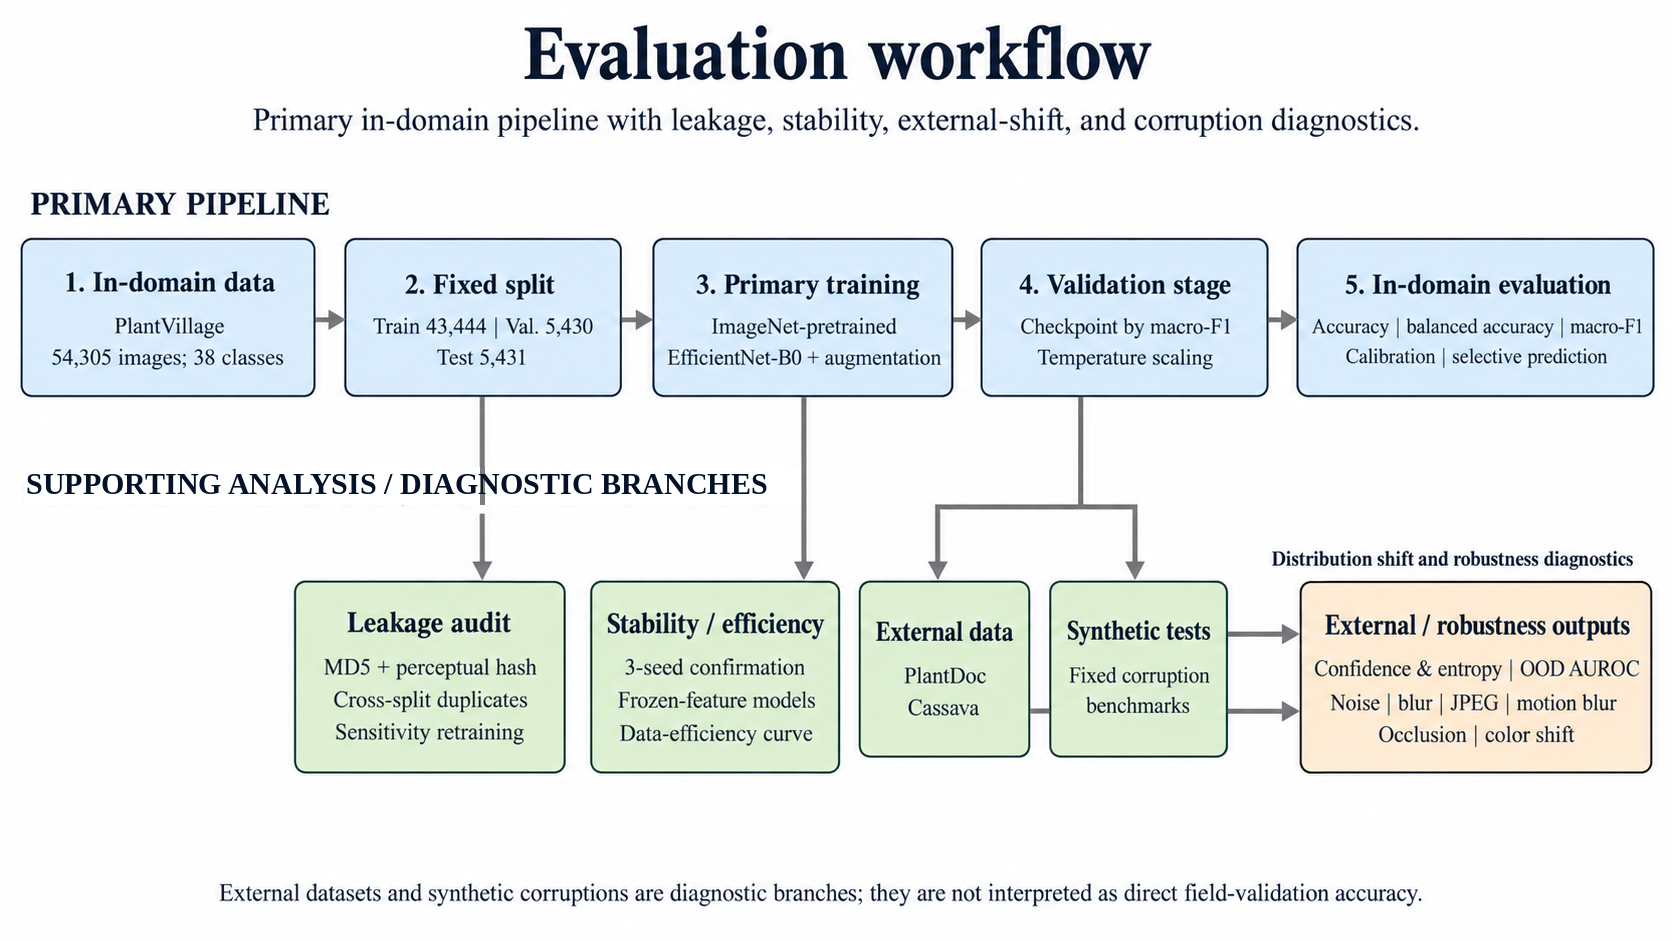
\includegraphics[width=0.98\textwidth]{figures/fig1_workflow.png}
\caption{Evaluation workflow. The primary in-domain pipeline is shown horizontally, while leakage auditing, stability and efficiency checks, external distribution-shift diagnostics, and synthetic corruption tests are treated as supporting branches. External OOD and corruption results are diagnostic rather than direct field-validation accuracy.}
\label{fig:workflow}
\end{figure*}


The EDA showed marked class imbalance in PlantVillage: the largest class contained 5,507 images and the smallest 152. The sample montages also differed visibly by dataset, with predominantly isolated leaves on controlled backgrounds in PlantVillage and more varied backgrounds and viewpoints in PlantDoc and Cassava. File-level auditing identified duplicate and near-duplicate matches, including seven exact duplicate groups that crossed the reconstructed train/validation/test boundaries and involved five test images. The leakage-aware sensitivity retraining used 5,426 unaffected test images and produced macro-F1 0.996191. The leakage-aware result is used as the conservative primary reference because it excludes the identified exact cross-split duplicates. The conventional fixed-split benchmark produced 0.997141 on 5,431 test images and is retained as a conventional benchmark comparison. Because the sensitivity run changed both training and test membership, the difference is descriptive rather than a direct causal estimate of leakage inflation. Representative EDA samples are shown in Fig.~\ref{fig:eda}. Dataset-count summaries are displayed in Fig.~\ref{fig:counts}.

\begin{figure*}[!t]
  \centering
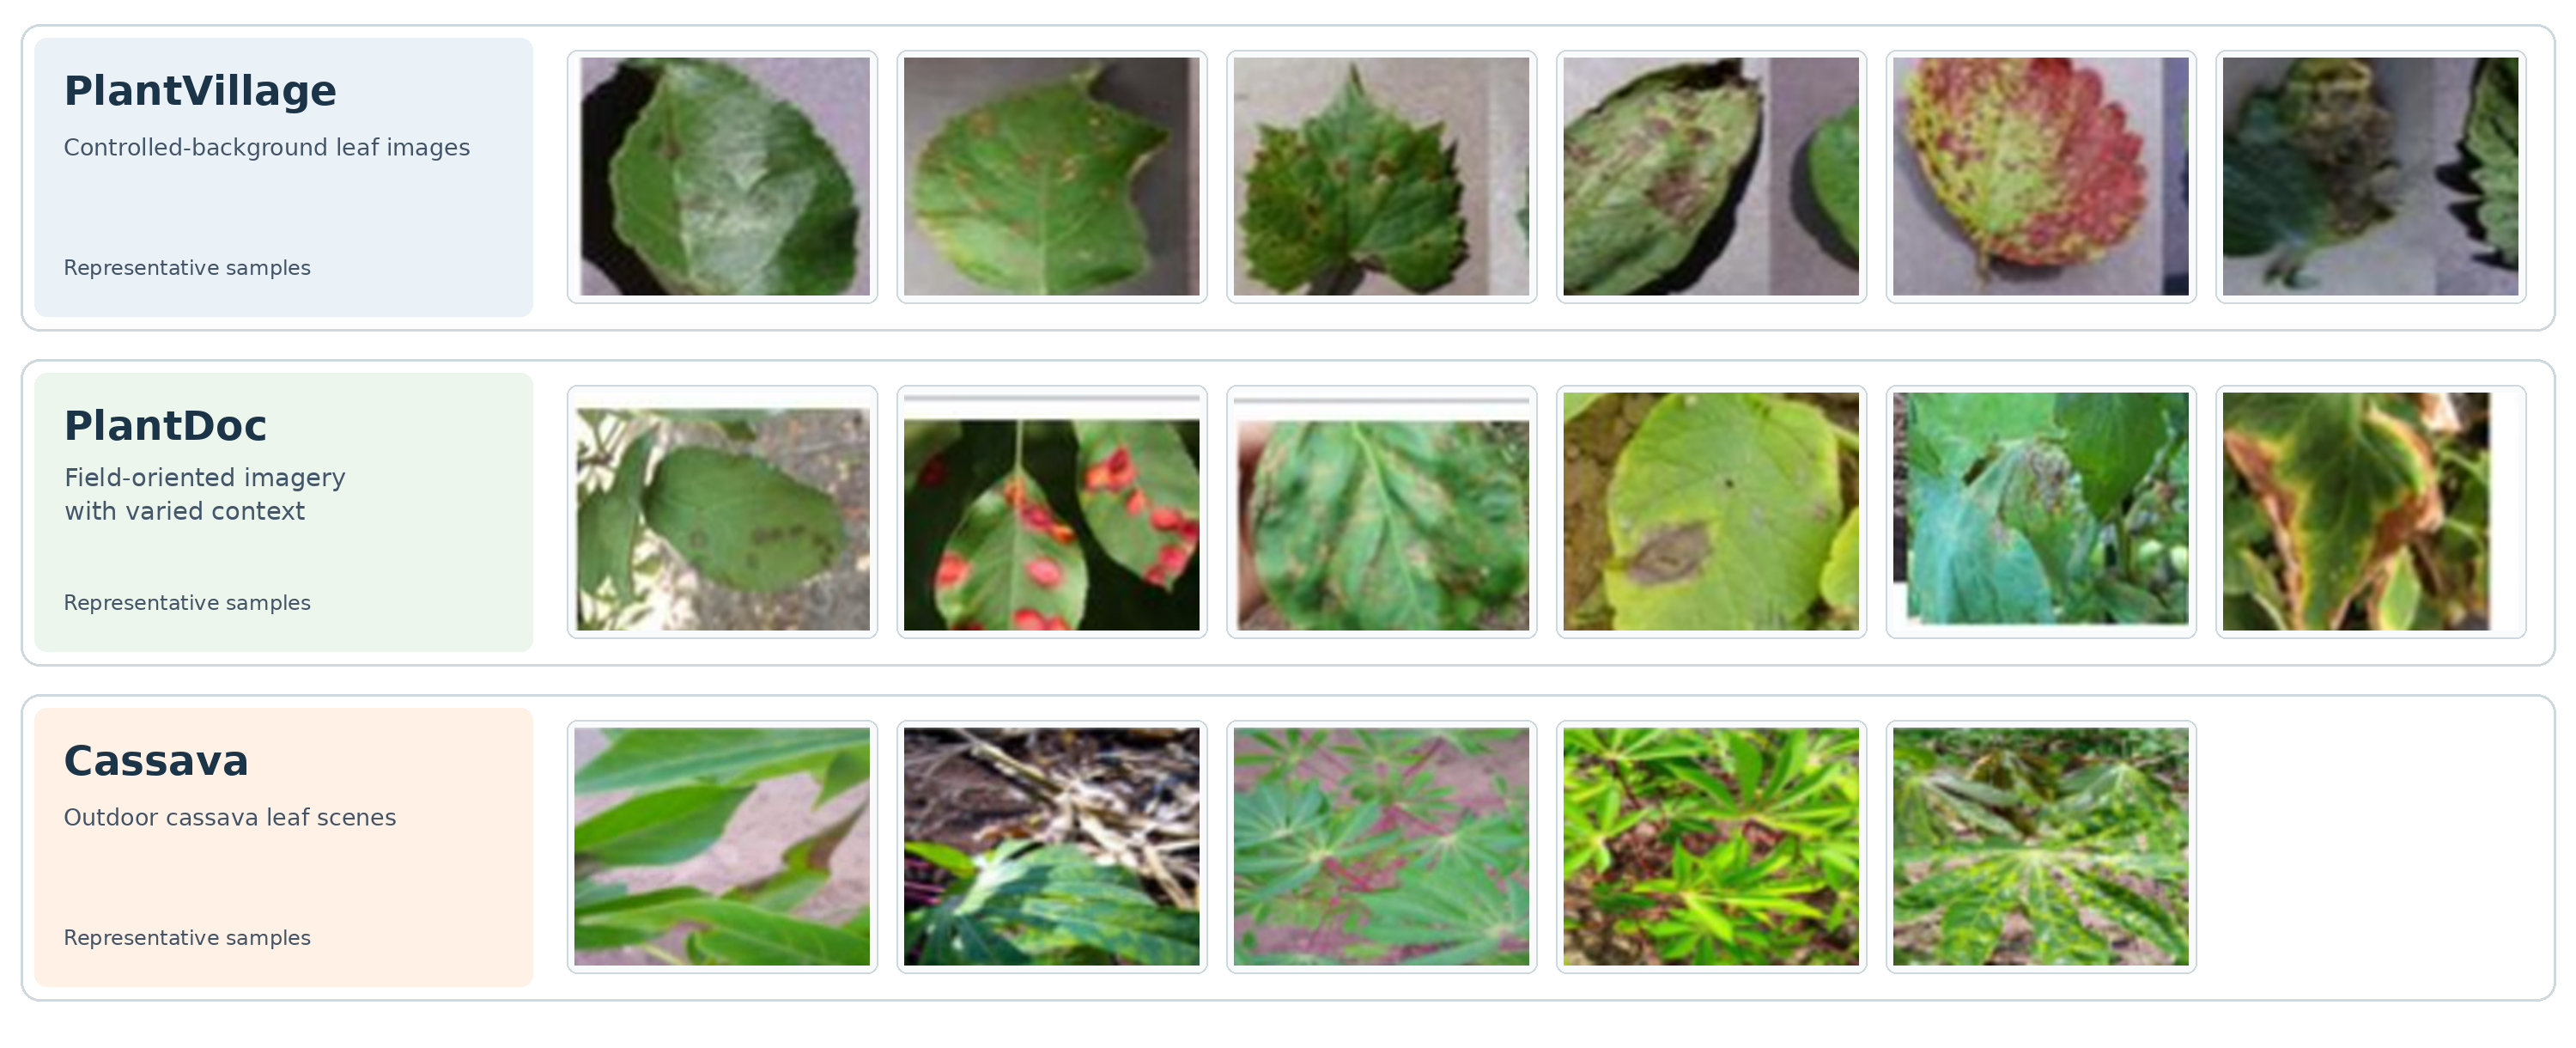
\includegraphics[width=0.98\textwidth]{figures/fig2_dataset_eda.png}
\caption{Qualitative examples of source-image crops from (top) PlantVillage, (middle) PlantDoc, and (bottom) Cassava, presented at a larger scale for legibility. Examples illustrate acquisition-context differences, not class frequency, severity, or diagnostic performance. Dataset counts and duplicate-audit statistics were calculated separately.}
\label{fig:eda}
\end{figure*}

\begin{figure*}[!t]
  \centering
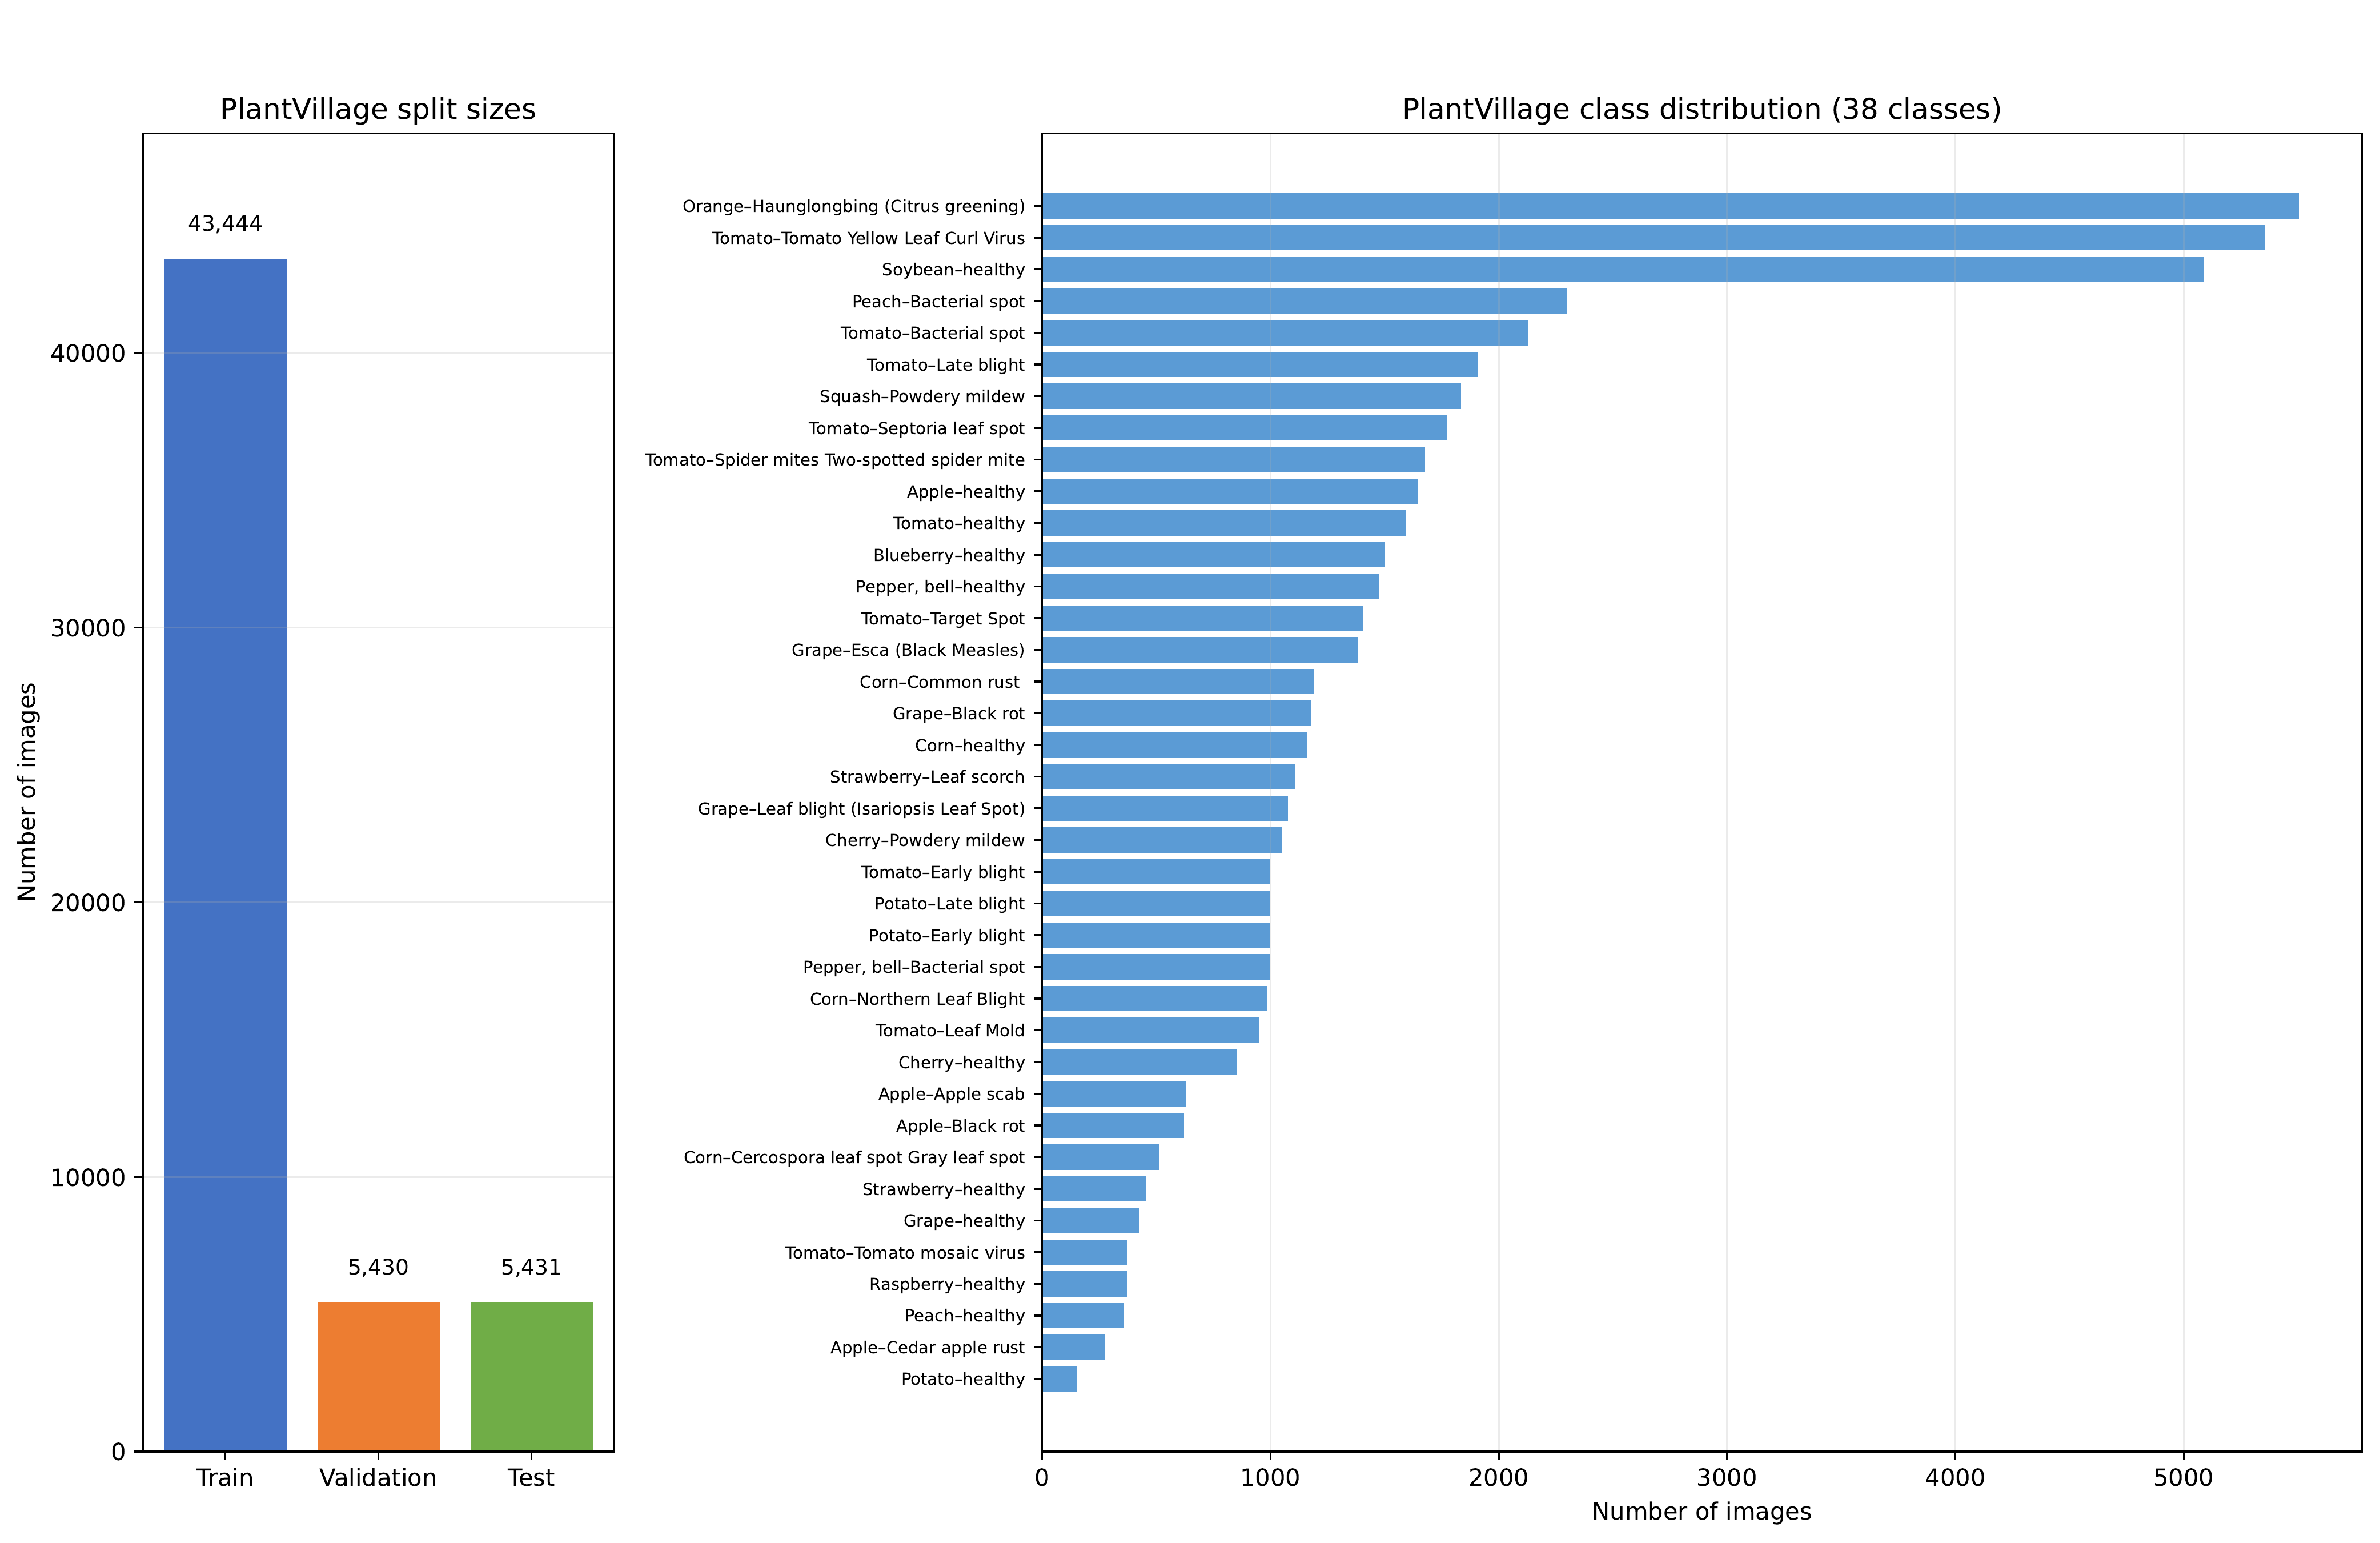
\includegraphics[width=0.94\textwidth]{figures/fig8_dataset_counts.png}
\caption{Dataset-count and class-frequency summaries used during exploratory analysis. The figure shows the observed class imbalance in the evaluated dataset copies and complements the representative image montage.}
\label{fig:counts}
\end{figure*}

\subsection{Recognition performance, calibration, and stability}
The EfficientNet-B0 basic-augmentation analysis achieved test accuracy 0.997975, balanced accuracy 0.996853, and macro-F1 0.997141. A separate locked primary rerun produced accuracy 0.998527, balanced accuracy 0.997470, and macro-F1 0.997808 with a 95\% sample bootstrap CI of [0.995955, 0.999251]. Mean maximum confidence was 0.786229 for PlantDoc and 0.881762 for Cassava. The original single-seed OOD AUROCs were 0.962139 and 0.939383, respectively. A corrected three-seed analysis using validation macro-F1 checkpoint selection gave PlantDoc AUROC mean 0.954748 (SD 0.020819) and Cassava AUROC mean 0.981930 (SD 0.017199). Pooled sample bootstrap 95\% CIs were [0.941144, 0.963795] for PlantDoc and [0.978510, 0.980477] for Cassava, hierarchical seed-by-sample CIs were [0.930746, 0.974009] and [0.962224, 0.992367], respectively. Because the external label spaces were not mapped to PlantVillage disease classes, these are distribution-shift and OOD diagnostics rather than external classification accuracy. Fig.~\ref{fig:perf_ood} summarizes the primary in-domain metrics and external diagnostics. The corresponding training history appears in Fig.~\ref{fig:training}.

\begin{figure*}[!t]
  \centering
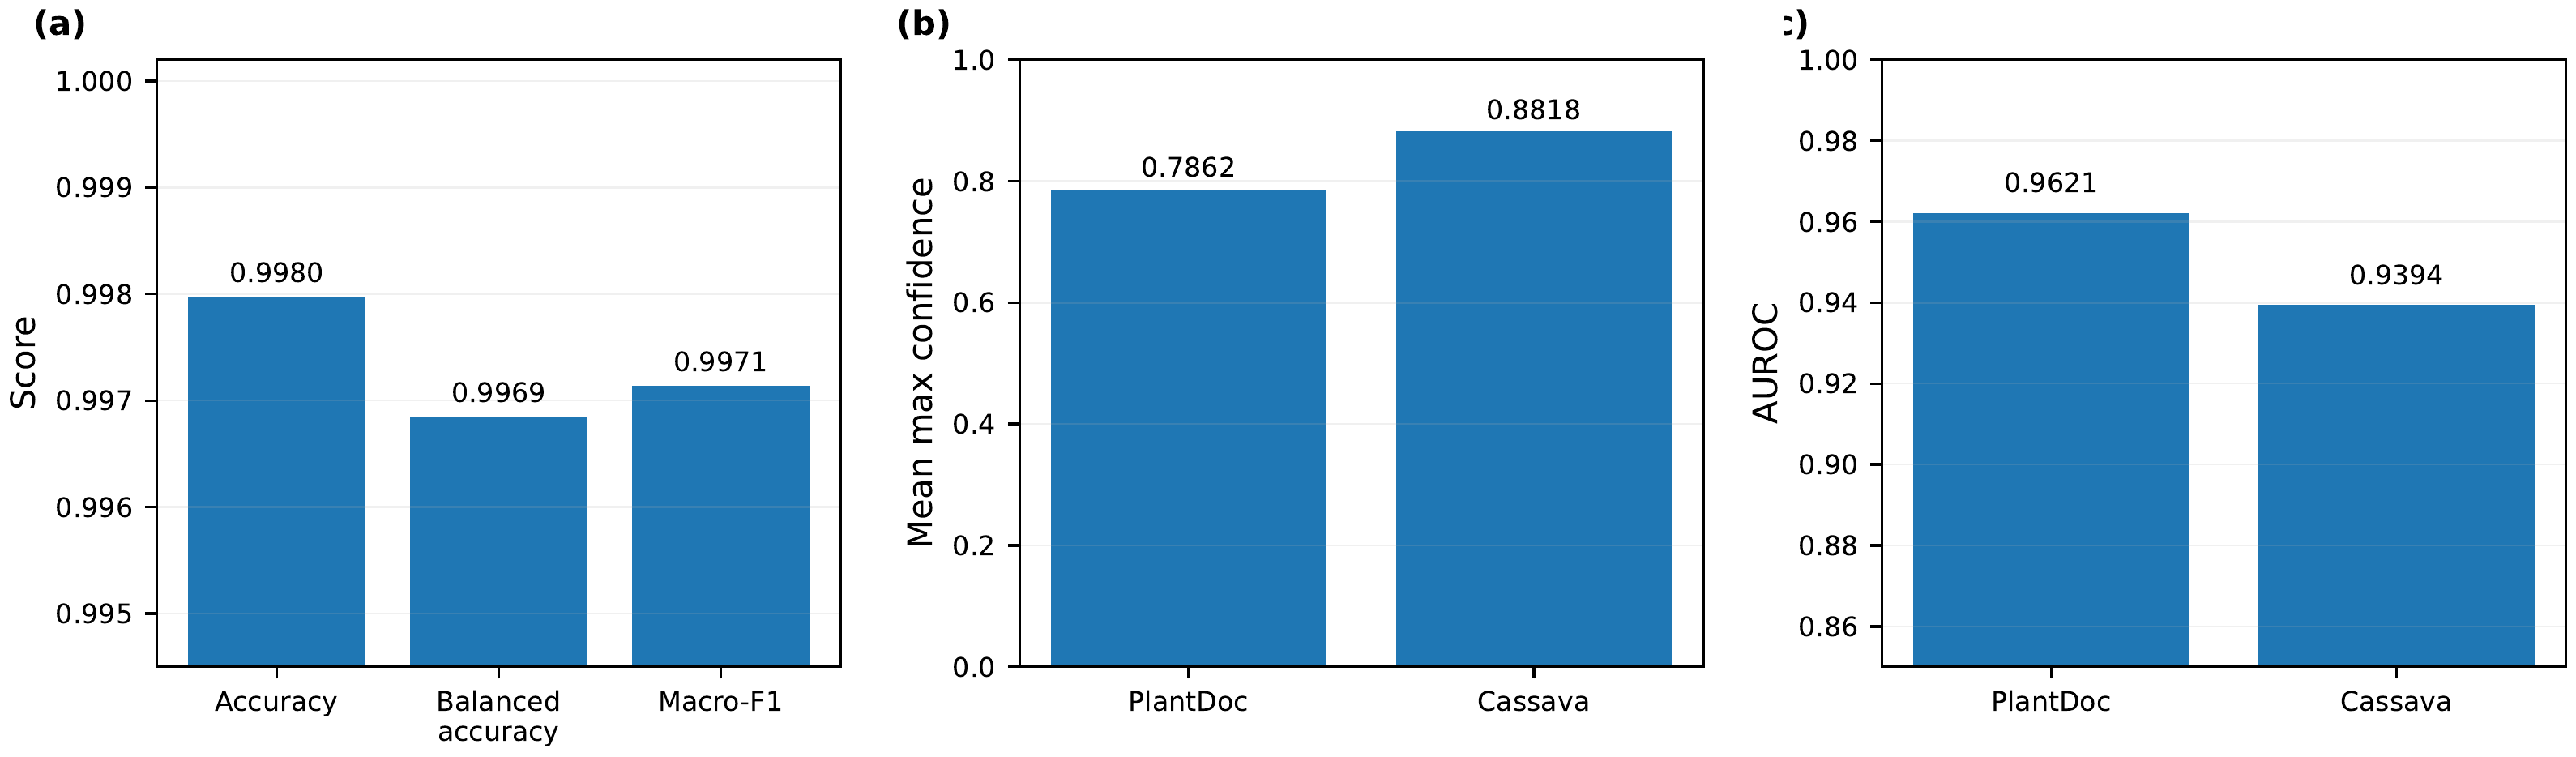
\includegraphics[width=0.98\textwidth]{figures/fig3_performance_and_ood.png}
\caption{Primary performance diagnostics. (a) EfficientNet-B0 in-domain test metrics on the fixed PlantVillage test split after validation-based checkpoint selection. (b) Mean maximum confidence on PlantDoc and Cassava. (c) OOD AUROC for the same external datasets. External confidence and OOD AUROC are distribution-shift diagnostics, not external disease-class accuracy.}
\label{fig:perf_ood}
\end{figure*}

\begin{figure*}[!t]
  \centering
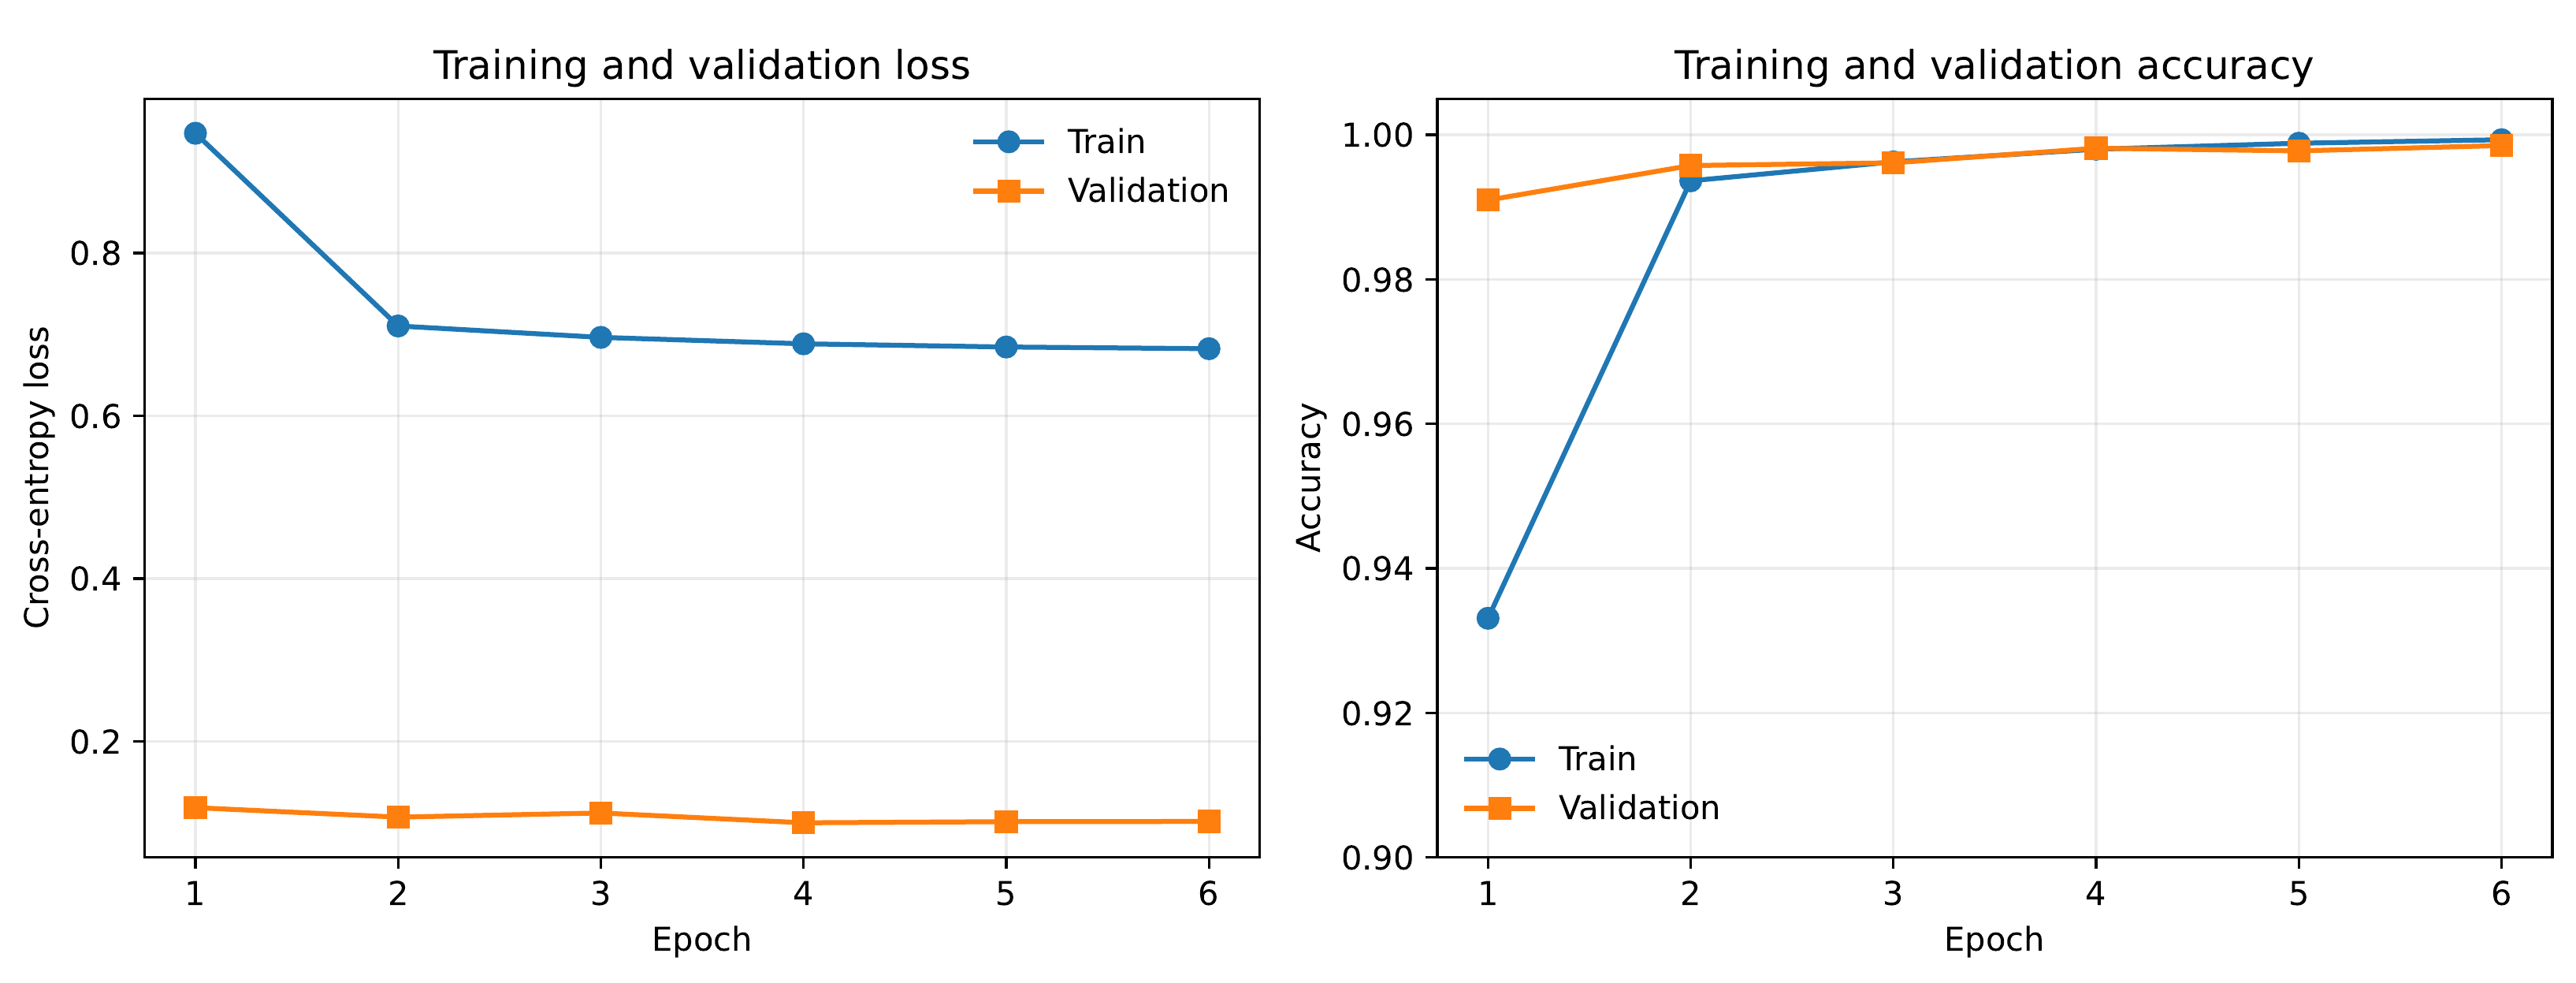
\includegraphics[width=0.97\textwidth]{figures/fig9_training_history.png}
\caption{Training history for the primary EfficientNet-B0 experiment. The curves are included to document the optimization trajectory associated with the selected checkpoint.}
\label{fig:training}
\end{figure*}


The locked primary report gives a fitted temperature of 0.517563 and test ECE 0.000876. A reproducibility rerun under the same documented protocol gave a fitted temperature of 0.517405 and test ECE 0.000878. In that rerun, test ECE decreased from 0.092371 to 0.000878, test NLL from 0.102458 to 0.007684, and test Brier score from 0.011559 to 0.002896. The separate primary rerun used for per-sample uncertainty had test ECE 0.001066 with a 95\% bootstrap CI of [0.000653, 0.002180]. The small difference between 0.000876 and 0.000878 reflects run-specific optimization and reporting provenance. The primary headline value remains 0.000876. Fig.~\ref{fig:calibration} shows the primary calibration summary and the rerun reliability bins.

\begin{figure*}[!t]
  \centering
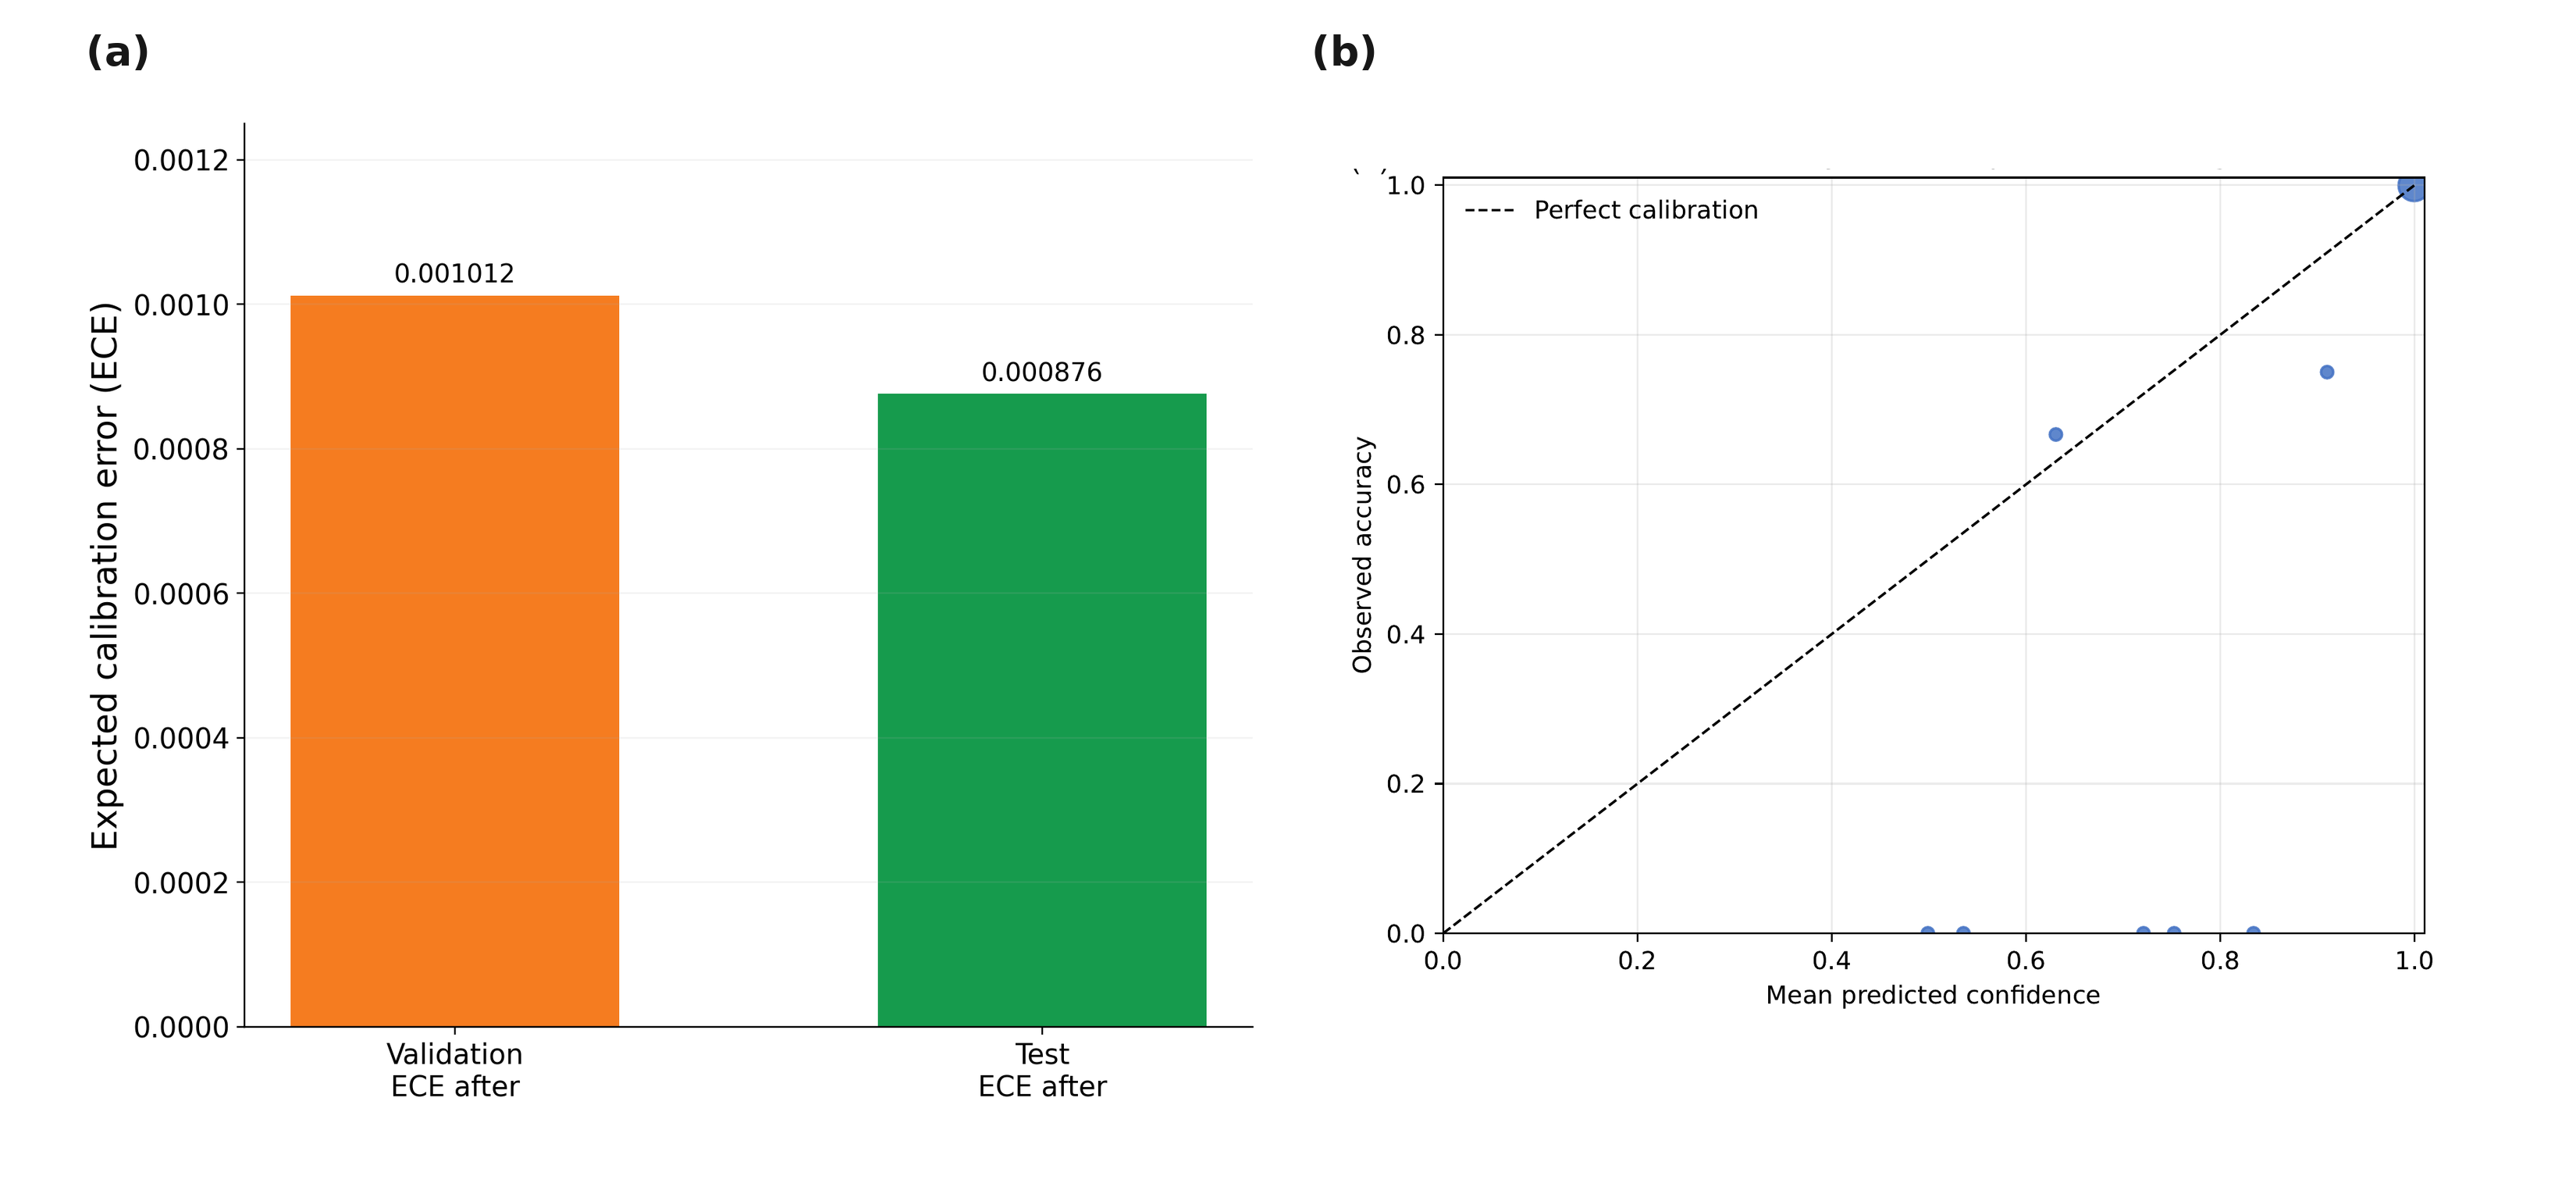
\includegraphics[width=0.97\textwidth]{figures/fig4_calibration_and_reliability.png}
\caption{Calibration diagnostics after validation-only temperature fitting. (a) In-domain ECE, with primary headline test ECE 0.000876 and independent rerun ECE 0.000878. (b) Test reliability bins from the rerun. Marker size is proportional to the number of observations in the bin.}
\label{fig:calibration}
\end{figure*}

At confidence thresholds 0.50, 0.80, 0.90, 0.95, and 0.99, the observed test coverages were 1.000000, 0.998711, 0.998159, 0.996686, and 0.994108, respectively. The corresponding accepted-sample macro-F1 values were 0.997141, 0.998523, 0.998689, 0.999650, and 0.999848. The per-sample primary rerun additionally gave bootstrap coverage intervals of [1.000000,1.000000], [0.997238,0.999263], [0.996133,0.998895], [0.995029,0.998159], and [0.990978,0.995213] at thresholds 0.50, 0.80, 0.90, 0.95, and 0.99, respectively. Its corresponding accepted-sample macro-F1 intervals were [0.995942,0.999228], [0.996856,0.999562], [0.997937,0.999860], [0.998114,1.000000], and [0.999506,1.000000].


Across seeds 7, 42, and 123, mean test accuracy was 0.998159 (standard deviation, SD, 0.000184), balanced accuracy 0.996725 (SD 0.000469), and macro-F1 0.997042 (SD 0.000522). Variation across the three runs was therefore small on the fixed split. The same stratified partition was reused for each seed, so these results assess stochastic training sensitivity only. They do not characterize robustness to alternative train/validation/test partitions or different farm-level sampling designs.

\begin{figure}[!tbp]
  \centering
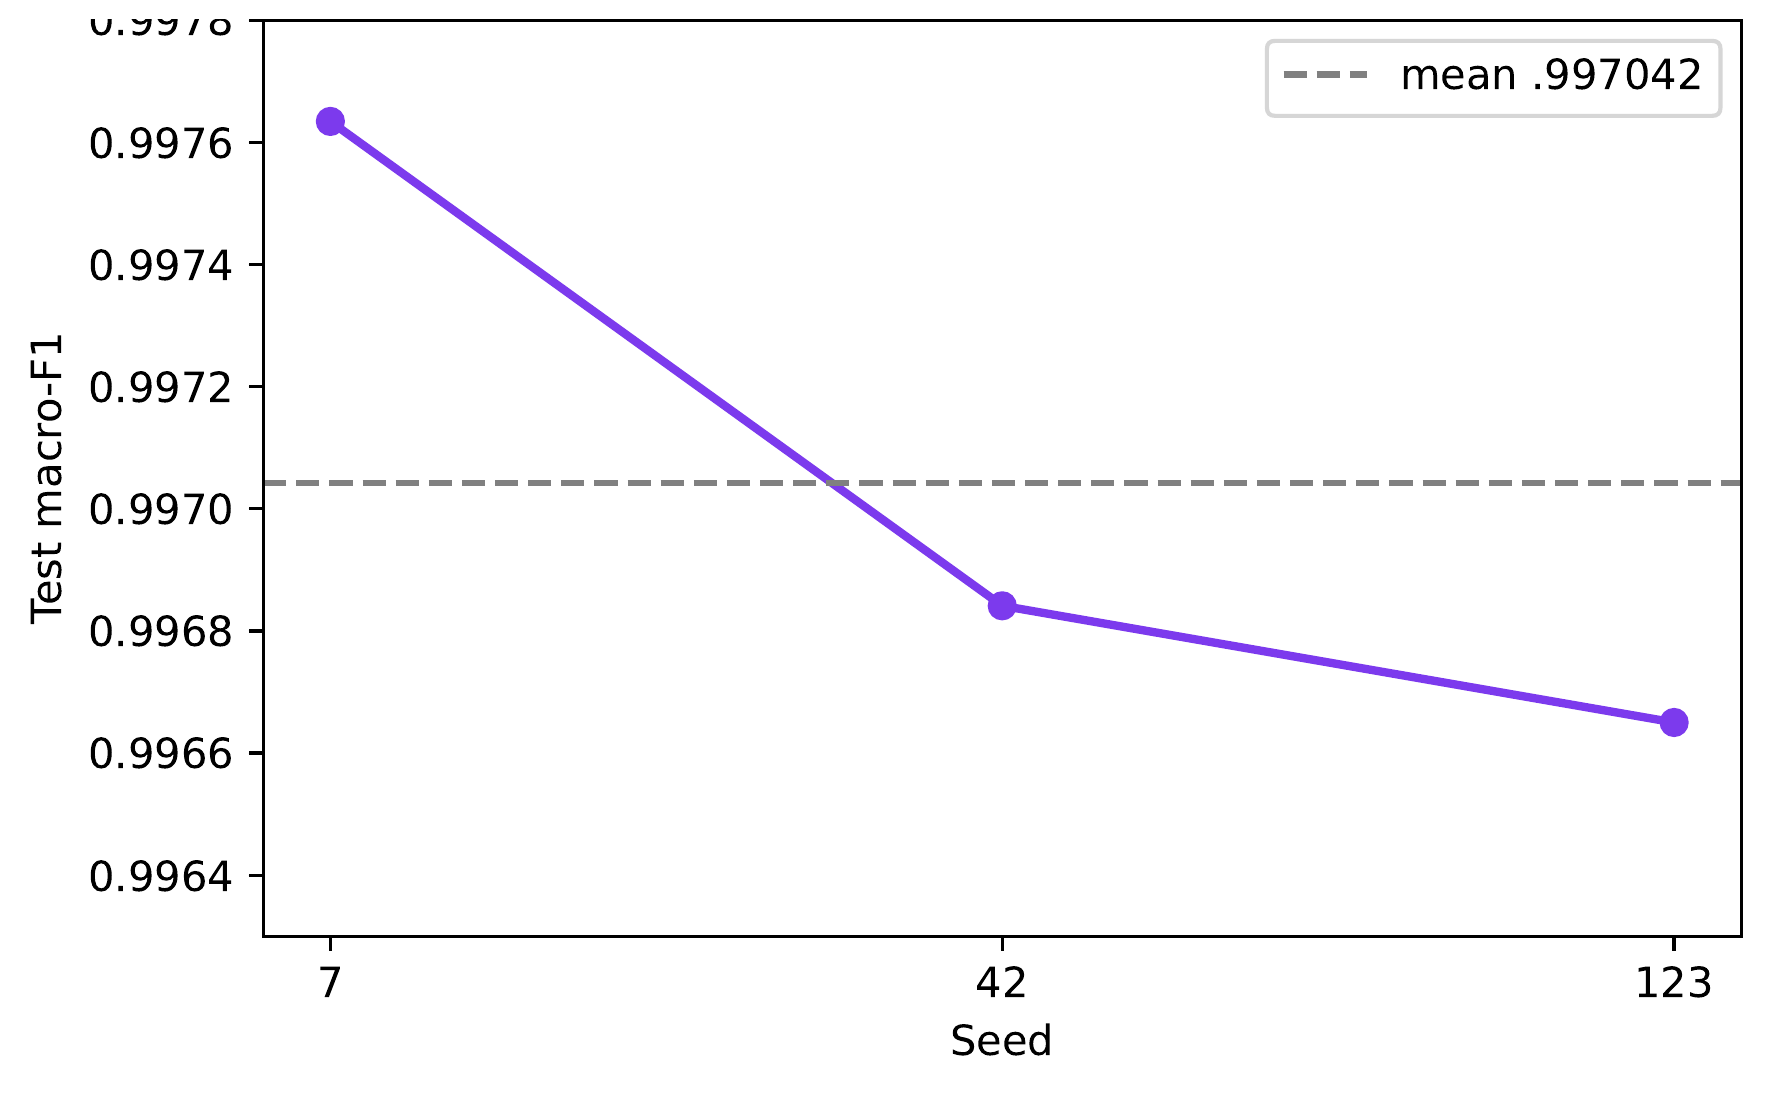
\includegraphics[width=0.98\columnwidth]{figures/fig5_seed_sensitivity.png}
\caption{Three-seed basic-augmentation confirmation. The dashed line denotes the descriptive mean. The plot does not represent a population-level confidence interval.}
\label{fig:seeds}
\end{figure}

\subsection{OOD evaluation and model/data efficiency}
The PlantDoc and Cassava AUROCs of 0.962139 and 0.939383 came from the original single-seed EfficientNet-B0 analysis using negative temperature-scaled maximum confidence. The corrected three-seed rerun used validation-only temperature fitting and validation macro-F1 checkpoint selection. It produced PlantDoc AUROC values of 0.972756, 0.959536, and 0.931952, with mean 0.954748 and SD 0.020819. Cassava values were 0.991935, 0.962071, and 0.991784, with mean 0.981930 and SD 0.017199. These values quantify run-to-run variability, while the seed-42 sample-level bootstrap gave PlantDoc 95\% CI [0.938322, 0.977221] and Cassava 95\% CI [0.959536, 0.964474]. The bootstrap intervals are conditional on that checkpoint and do not isolate dataset-sampling uncertainty across alternative external mirrors. They should not be compared directly with an earlier energy-versus-MSP diagnostic, which used a two-epoch seed-42 checkpoint, calibration and evaluation halves of each external dataset, and different scores. In that separate analysis, energy AUROC was 0.8682 and MSP AUROC was 0.8429, with energy OOD TPR 0.9496 and in-domain FPR 0.5113. Neither experiment measures external disease-class accuracy.

In the frozen-feature model-family benchmark, test macro-F1 was 0.9708 for ResNet-50, 0.9702 for MobileNetV3-Large, and 0.9714 for EfficientNet-B0. The paired accuracy intervals included zero for every comparison. The intervals were [-0.001846, 0.006813] for ResNet-50 versus MobileNetV3-Large, [-0.004235, 0.004055] for ResNet-50 versus EfficientNet-B0, and [-0.007001, 0.001841] for MobileNetV3-Large versus EfficientNet-B0. The reported intervals were formed from 1,000 paired bootstrap replicates on a common test set. All three accuracy-difference intervals include zero. An additional paired macro-F1 bootstrap using 5,000 identical-index resamples gave 95\% intervals of [0.963686, 0.976603] for ResNet-50, [0.963335, 0.975846] for MobileNetV3-Large, and [0.964838, 0.976803] for EfficientNet-B0. The paired macro-F1 differences were 0.000627 for ResNet-50 versus MobileNetV3-Large (95\% CI [-0.007103, 0.007980]), -0.000642 for ResNet-50 versus EfficientNet-B0 (95\% CI [-0.008037, 0.006263]), and -0.001269 for MobileNetV3-Large versus EfficientNet-B0 (95\% CI [-0.008397, 0.005779]). These intervals are conditional on the common test set and do not quantify variability across independently collected farms or training conditions. The corresponding model-family comparison is shown in Fig.~\ref{fig:family}.

\begin{figure}[!tbp]
  \centering
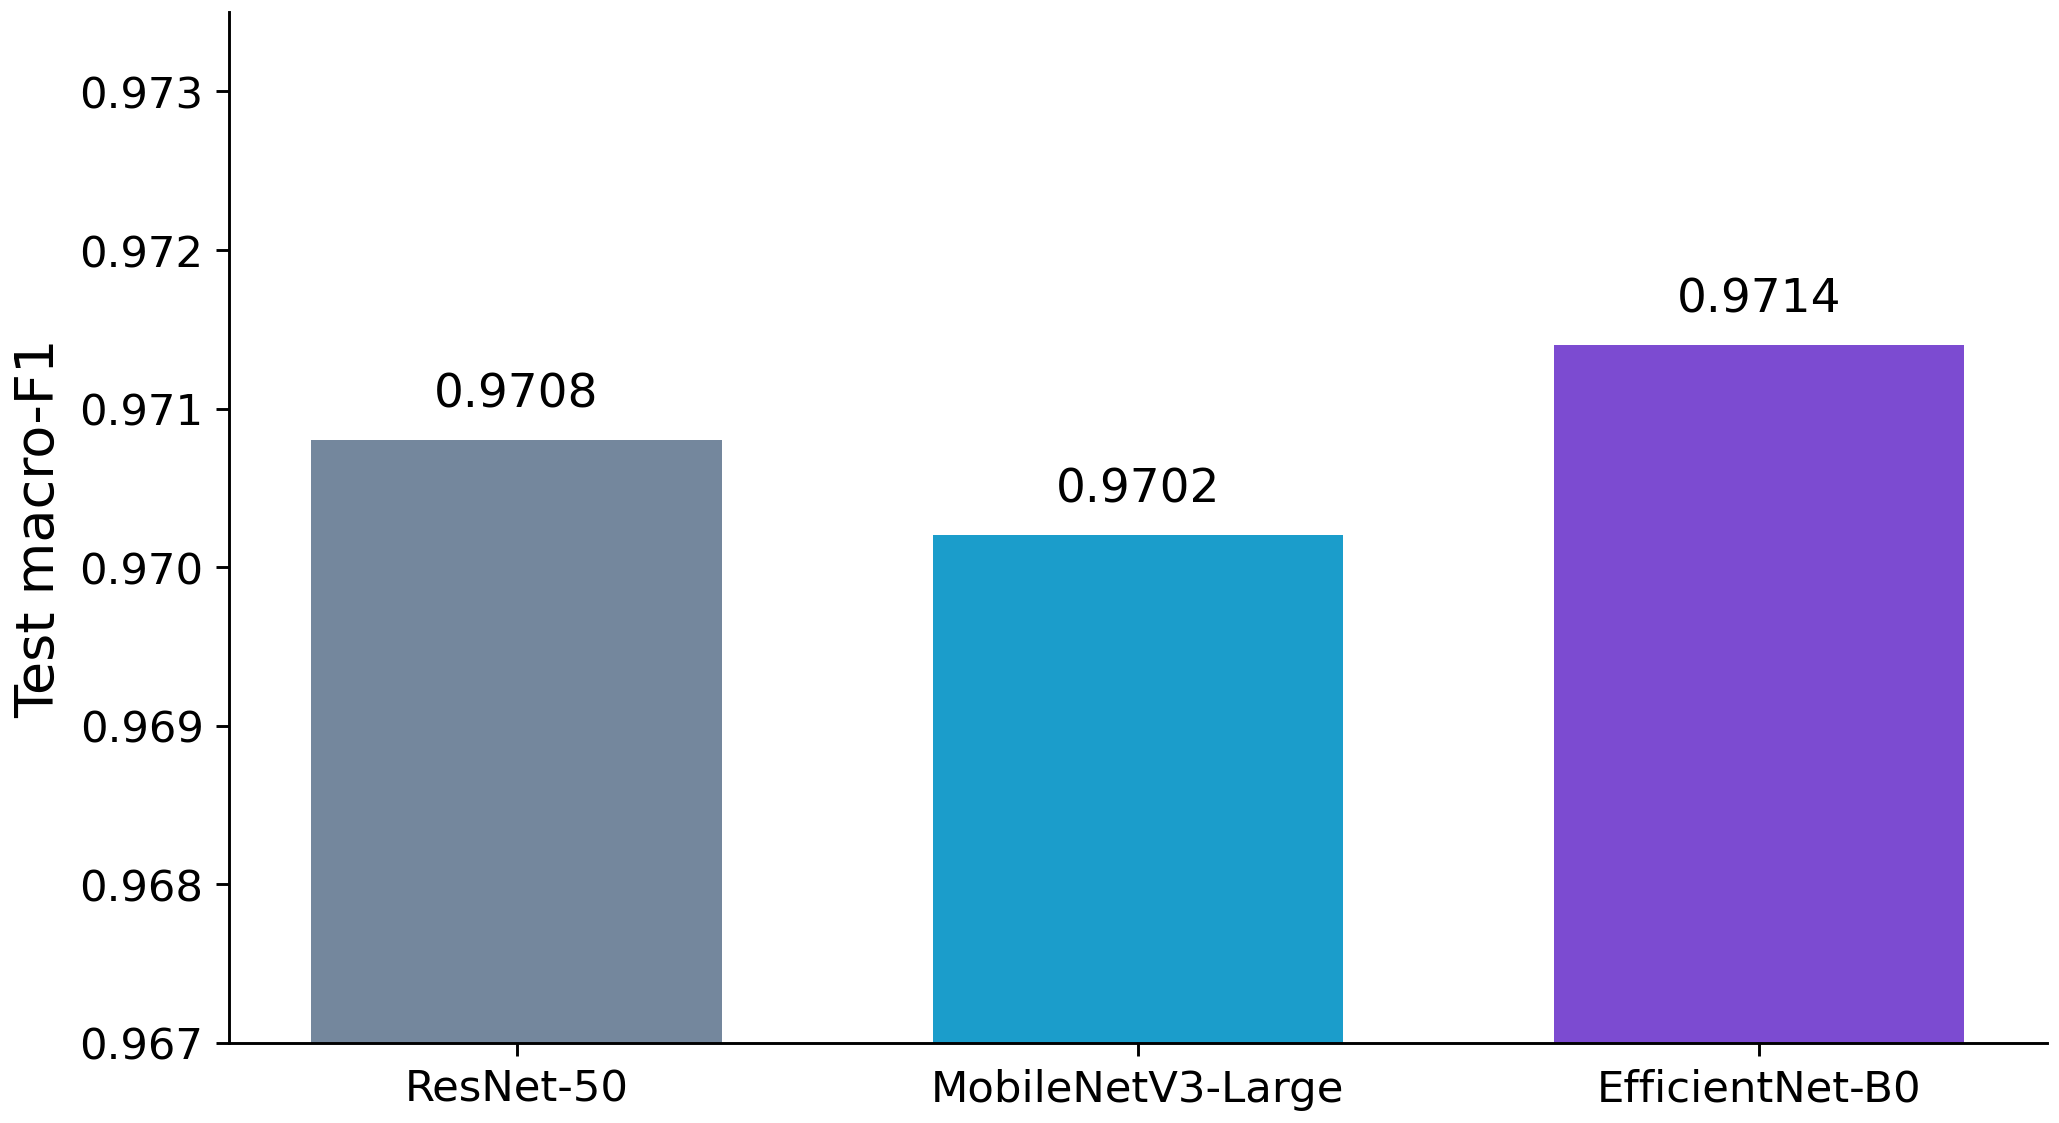
\includegraphics[width=0.80\columnwidth]{figures/fig10_model_family.png}
\caption{Frozen-feature model-family comparison. Bars summarize descriptive macro-F1 results under the common frozen-feature protocol. Paired intervals reported in the text do not establish a statistically supported winner.}
\label{fig:family}
\end{figure}


Test macro-F1 was 0.7193 with 1\%, 0.8789 with 5\%, 0.9128 with 10\%, 0.9438 with 25\%, 0.9602 with 50\%, and 0.9668 with 100\% of the training data in the frozen-feature protocol. The largest absolute increase occurred between 1\% and 5\% (0.1596), followed by 5\% to 10\% (0.0339). The increase from 10\% to 100\% was smaller (0.0540), as shown in Fig.~\ref{fig:dataeff}.

\begin{figure}[!tbp]
  \centering
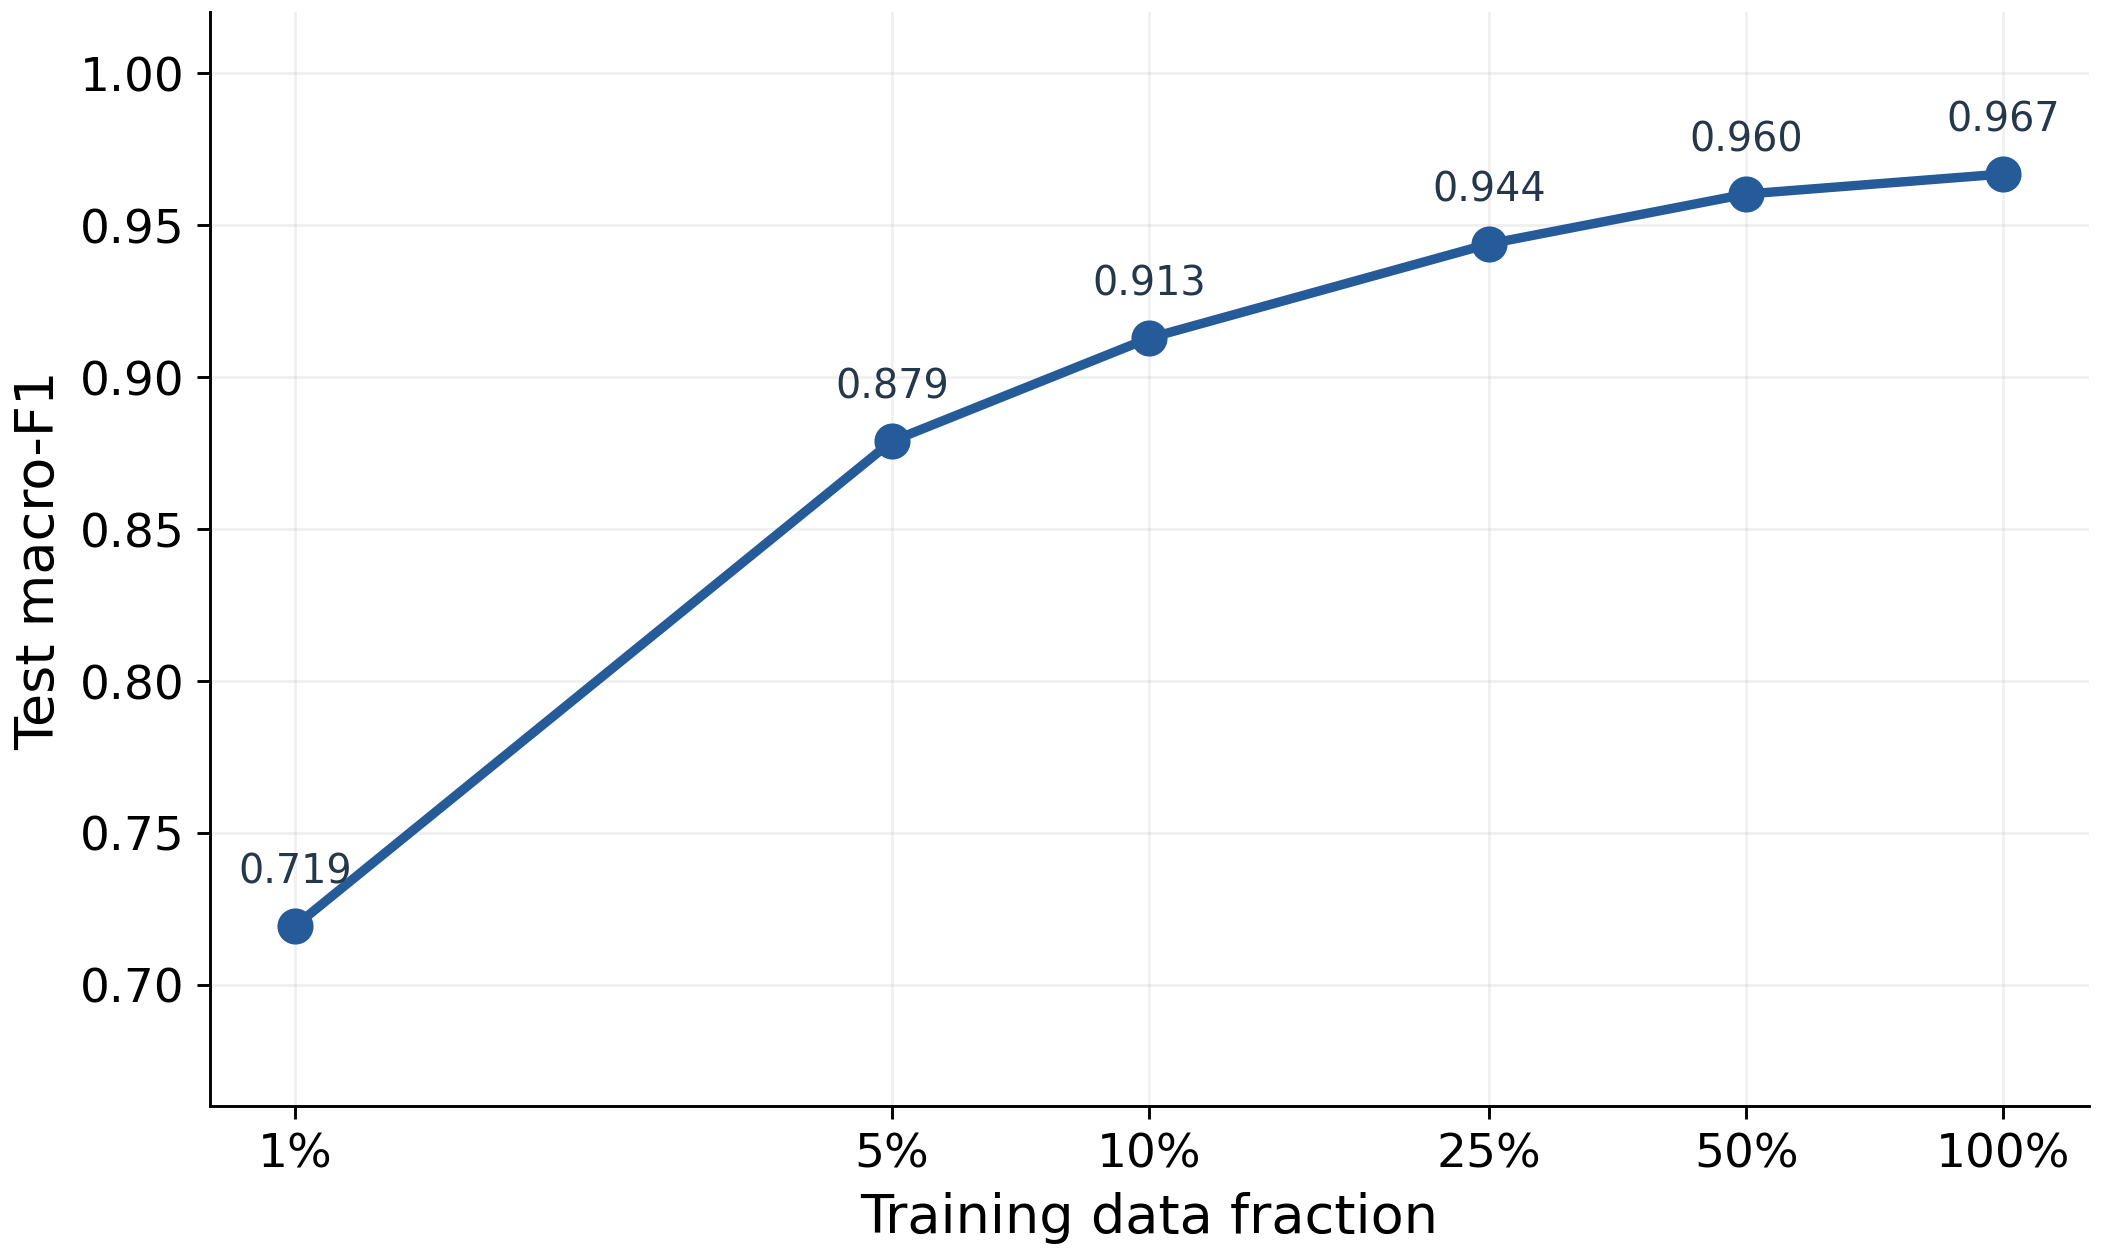
\includegraphics[width=0.98\columnwidth]{figures/fig6_data_efficiency.png}
\caption{Data-efficiency curve for the frozen ResNet-50 feature protocol. The logarithmic horizontal axis emphasizes the low-data region.}
\label{fig:dataeff}
\end{figure}


\subsection{Computational efficiency}
The model-only GPU benchmark measured mean latency per image of 2.9255~ms for ResNet-50, 0.6602~ms for MobileNetV3-Large, and 1.1229~ms for EfficientNet-B0. Peak allocated memory was 443.791, 269.149, and 369.692~MiB, respectively. These results are protocol-specific measurements on a Tesla T4 and exclude preprocessing, data transfer, and postprocessing.

\begin{table}[!tbp]
\centering
\caption{Model-only GPU inference benchmark on a Tesla T4. Latency excludes preprocessing, data transfer, and postprocessing.}
\label{tab:compute_benchmark}
\small
\begin{tabular}{lrr}
\toprule
Model & Latency/image (ms) & Peak memory (MiB) \\
\midrule
ResNet-50 & 2.9255 & 443.791 \\
MobileNetV3-Large & 0.6602 & 269.149 \\
EfficientNet-B0 & 1.1229 & 369.692 \\
\bottomrule
\end{tabular}
\end{table}

\subsection{Corruption-specific robustness}
The paired unseen-corruption comparison showed a specific pattern. The basic and blur-aware models achieved clean macro-F1 values of 0.998250 and 0.993473, respectively. On JPEG compression, macro-F1 was 0.970985 for the basic model and 0.973621 for the blur-aware model. Motion-blur macro-F1 increased from 0.428671 to 0.901282 with blur-aware training. In contrast, square-occlusion macro-F1 decreased from 0.981667 to 0.965052, and red-channel color-shift macro-F1 decreased from 0.672191 to 0.625801. The large gain was therefore specific to motion blur: JPEG changed little, while square occlusion and red-channel color shift became worse after blur-aware training. A separate retained per-sample rerun gave paired bootstrap 95\% CIs for the blur-aware minus basic macro-F1 difference of [-0.002038, 0.003082] on clean images, [0.014096, 0.027512] under JPEG, [0.440244, 0.475648] under motion blur, [-0.004310, 0.005843] under occlusion, and [-0.103377, -0.071513] under color shift. These intervals are conditional on that rerun and protocol. They do not establish generalization to unseen corruption families.

\begin{table}[!tbp]
  \centering
  \caption{Within-protocol macro-F1 differences (blur-aware minus basic model) from the original paired run. These point estimates are reported separately from the retained-prediction bootstrap intervals in the text.}
  \label{tab:paired_effects}
  \small
  \begin{tabular}{lr}
  \toprule
  Test condition & $\Delta$ macro-F1 \\
  \midrule
  Clean & $-0.004777$ \\
  JPEG compression & $+0.002636$ \\
  Motion blur & $+0.472611$ \\
  Square occlusion & $-0.016615$ \\
  Red-channel shift & $-0.046390$ \\
  \bottomrule
  \end{tabular}
\end{table}

The corruption-aware single-run model had clean-test macro-F1 0.996473, compared with 0.997141 for the basic model. Under the matched Gaussian-noise and blur tests, it achieved macro-F1 0.991162 and 0.994484 in the single reported run. Across three exploratory runs, the corresponding means were 0.992783 and 0.993981. The clean-test difference was 0.000668. The different corruption protocols and their metrics are consolidated in Table~\ref{tab:corruption_protocols}. Values should not be pooled because the training augmentations, checkpoints, or evaluation transformations differ.

\begin{table*}[!tbp]
  \centering
\caption{Macro-F1 across corruption protocols. N/A denotes transformations not evaluated in that protocol. The additional basic evaluation used a separate run from the paired experiment, explaining its different values.}
\label{tab:corruption_protocols}
\small
\begin{tabular}{lrrrrrrr}
\toprule
Protocol & Clean & Noise & Blur & JPEG & Motion & Occl. & Color \\
\midrule
Primary basic & 0.9971 & 0.4057 & 0.4707 & N/A & N/A & N/A & N/A\\
Matched corruption-aware & 0.9965 & 0.9912 & 0.9945 & N/A & N/A & N/A & N/A\\
Paired basic & 0.9983 & N/A & N/A & 0.9710 & 0.4287 & 0.9817 & 0.6722\\
Paired blur-aware & 0.9935 & N/A & N/A & 0.9736 & 0.9013 & 0.9651 & 0.6258\\
Additional basic evaluation & N/A & N/A & N/A & 0.9727 & 0.4452 & 0.9783 & 0.6657\\
\bottomrule
\end{tabular}
\end{table*}

\begin{figure}[!tbp]
  \centering
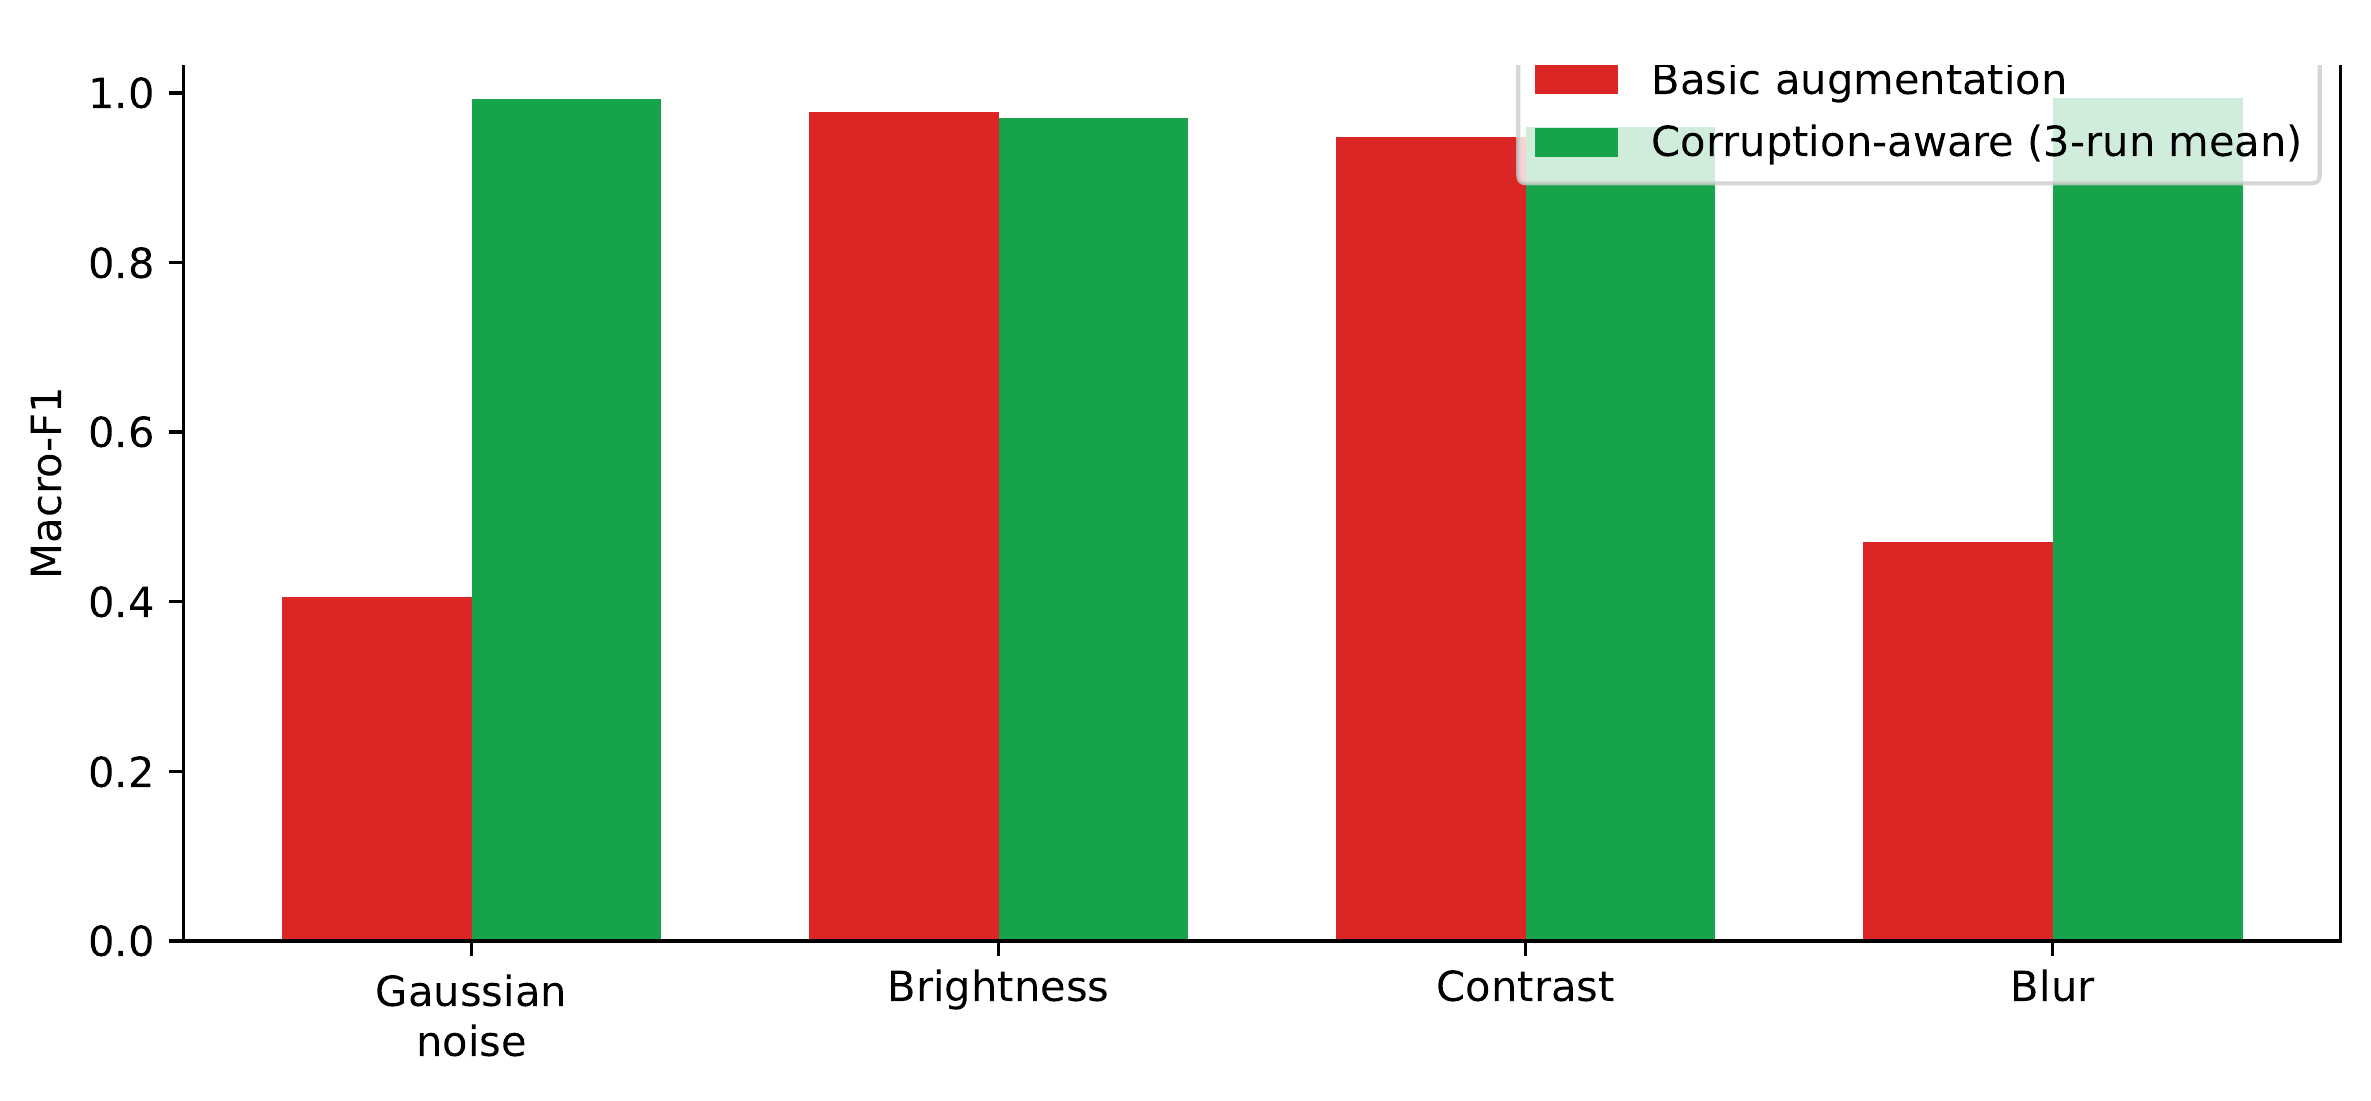
\includegraphics[width=0.86\columnwidth]{figures/fig7_corruption.png}
\caption{Synthetic corruption robustness diagnostic. Basic and corruption-aware results use separate training protocols. The corruption-aware multi-run bars are descriptive means.}
\label{fig:corruption}
\end{figure}

\section{Discussion}\label{sec:discussion}
\subsection{Benchmark performance, leakage, and dataset shift}
The primary EfficientNet-B0 experiment produced near-ceiling performance on the fixed PlantVillage test split. That result is useful as an in-domain reference, but it should be interpreted in the context of how PlantVillage was constructed. The original PlantVillage release describes a large, expertly curated leaf-image repository intended to support machine-learning diagnosis \cite{r01}. PlantDoc, by contrast, was introduced to increase the availability of non-laboratory images and therefore represents a visibly different acquisition regime \cite{r02}.

The external observations address score separation between known PlantVillage images and two heterogeneous dataset mirrors. They do not establish disease-recognition accuracy in field conditions. Differences in backgrounds and illumination coexist with changes in crop species, disease labels, collection sources, and image-selection policies. In particular, a high OOD AUROC can be driven by recognition of dataset origin or semantic mismatch without demonstrating any useful field diagnosis. The external confidence results are consistent with the broader cross-dataset literature. Mahapatra et al. reported a clear gap between their strongest intra-dataset and cross-dataset results across several plant-disease datasets \cite{r39}. Zhang and Liu also treated PlantDoc as a challenging field-acquired dataset with complex backgrounds and designed their model around those difficulties \cite{r14}. For that reason, the PlantDoc and Cassava results in this study are interpreted as distribution-shift diagnostics rather than disease-class transfer accuracy.

The duplicate audit found seven exact cross-split groups involving five training, four validation, and five test images. Near-identical images indicated by nonzero perceptual-hash distances were identified but not removed by the exact-MD5 sensitivity analysis. After excluding the 14 exact-duplicate images and retraining, macro-F1 was 0.996191 on an unaffected test subset rather than 0.997141 on the original test set. Because both training membership and evaluated test membership changed, this is a sensitivity result and not an isolated causal estimate of leakage inflation. Protocol transparency is equally important: the fine-tuning, calibration, OOD, frozen-feature, and corruption-aware results are kept separate because they do not all come from the same checkpoint.

\subsection{Calibration and corruption-specific robustness}
The validation-fitted temperature reduced the primary test ECE to 0.000876, while an independent rerun produced 0.000878. Both ECE values are conditional on the curated PlantVillage distribution and 15-bin evaluation. Calibration on validation images from that source cannot be presumed stable under the visual and semantic shifts observed in PlantDoc and Cassava, especially when external labels are incompatible. External-dataset calibration error was therefore not evaluated. This use of a single validation-fitted temperature follows the post-hoc calibration principle studied by Guo et al. \cite{r04}. Balanya et al. later showed that temperature can be made input-dependent and that simpler entropy-informed scaling can be attractive when calibration data are limited \cite{r21}. The present study deliberately retains the simpler scalar-temperature setting so that the calibration protocol remains easy to reproduce.

Selective prediction also changed the interpretation of accuracy. As the confidence threshold increased, coverage decreased slightly while accepted-sample macro-F1 increased. This pattern describes confidence ranking on the fixed in-domain test set. It is not evidence that the same threshold would remain optimal after a domain shift. More general uncertainty methods, such as prediction intervals trained with selective joint supervision, show that uncertainty estimation is itself a modeling problem rather than a direct consequence of high classification accuracy \cite{r25}.

The corruption experiments show that augmentation effects were specific to the perturbation being tested. The basic model was sensitive to strong Gaussian noise and blur, whereas matched corruption-aware training recovered much of that performance. Enkvetchakul and Surinta likewise reported that particular geometric augmentation combinations improved recognition in their plant-leaf setting \cite{r06}. Lee and Lee found benefits from geometric and color-space augmentation on a broader crop-disease dataset \cite{r27}. Neither result implies that one augmentation policy should improve every unseen corruption.

The paired blur-aware experiment illustrates this limitation directly. Motion-blur macro-F1 increased from 0.4287 to 0.9013, but red-channel color shift and square occlusion worsened. Mitra et al. studied corruption robustness and calibration as separate safety properties in image classifiers \cite{r07}. Park et al. similarly treated corruption robustness as an adaptation problem and used test-time training on corrupted images \cite{r11}. The present results therefore support perturbation-specific reporting rather than a single generic robustness label.

\subsection{Model efficiency, data efficiency, and limitations}
The frozen-feature benchmark yielded only small descriptive differences among ResNet-50, MobileNetV3-Large, and EfficientNet-B0, and every paired interval crossed zero. A separate model-only inference benchmark on a Tesla T4 runtime measured mean per-image latencies of 2.9255 ms, 0.6602 ms, and 1.1229 ms for ResNet-50, MobileNetV3-Large, and EfficientNet-B0, respectively, with peak allocated memory of 443.791, 269.149, and 369.692 MiB. These measurements use random 224$\times$224 inputs, batch size 32, 20 warm-up iterations, and 100 CUDA-event timed iterations. They describe one current runtime and are not time-matched evidence about the historical Phase 58 training hardware. They also do not measure energy or deployment throughput under application workloads. Zheng et al. document the diversity of RGB and spectral crop-disease recognition approaches in their recent survey \cite{r38}. The model-family performance and runtime measurements should therefore be read as protocol-specific comparisons rather than evidence of universal computational superiority.

The data-efficiency experiment adds another practical perspective. Macro-F1 improved rapidly between 1\% and 10\% of the training data and then increased more gradually as the training fraction grew. This pattern is specific to frozen ResNet-50 features and the sampled PlantVillage split, but it helps separate representation reuse from full-model fine-tuning. It also provides a reproducible reference for future work that may compare field datasets or stronger self-supervised representations.



The study does not provide a prospective farm-level validation. The evaluated mirrors did not include farm, cultivar, season, device, or disease-severity metadata, so the evaluation cannot estimate variation across farms, cultivars, acquisition sessions, camera hardware, growing seasons, or disease stages. Their absence also prevents source-group-disjoint splitting, confounder adjustment, and checks for whether visually similar images were captured during one session. Thus, even the leakage-aware PlantVillage score cannot be extrapolated quantitatively to new farms or disease severities. DiaMOS Plant illustrates how diagnosis and monitoring datasets can move beyond a single disease label by including disease-severity levels and fruit-growth stages \cite{r41}. Future validation should similarly preserve acquisition metadata so that field generalization can be tested directly.

The external datasets were also not label-harmonized with PlantVillage. Consequently, the OOD analysis evaluates unfamiliarity rather than cross-dataset disease accuracy. Li et al. emphasize that OOD benchmarks can combine semantic and domain shifts, particularly when sensors or spatial distributions differ \cite{r42}. A stronger follow-up study would predefine a shared disease taxonomy and collect matched observations across farms, devices, cultivars, and disease stages.
\section{Conclusions}\label{sec:conclusion}
This study evaluated crop-disease recognition beyond a single random-split score. The exact-duplicate-exclusion retraining achieved macro-F1 0.996191 on 5,426 unaffected test images, while a stricter full group-deduplication sensitivity run achieved macro-F1 0.996661 on 5,316 test images. The conventional EfficientNet-B0 model achieved macro-F1 0.997141 on the fixed 5,431-image PlantVillage test split. These in-domain results use different partition memberships and are descriptive sensitivity comparisons, not causal estimates of leakage. Across three independent seeds, external OOD AUROC averaged 0.954748 (SD 0.020819) for PlantDoc and 0.981930 (SD 0.017199) for Cassava. Both results are OOD diagnostics rather than external disease-class accuracy and do not establish field deployment readiness. The wider evaluation identified several qualifications: calibration required validation-fitted temperature scaling, robustness gains depended on the corruption being tested, and runtime measurements were obtained on a separate current GPU environment. The three-seed confirmation and computational benchmark therefore complement, rather than replace, the protocol-specific in-domain and distribution-shift evaluations.

Taken together, the results support a reporting strategy in which in-domain accuracy, leakage auditing, calibration, OOD behavior, selective prediction, seed variation, and corruption robustness are presented as distinct quantities. The next validation step should use pre-specified group-disjoint field data with shared disease labels and acquisition metadata. The present PlantVillage results do not demonstrate generalization to real field conditions because no prospective field validation, matched-label cross-dataset accuracy evaluation, or farm-disjoint deployment study was performed. A future design with shared disease labels, acquisition metadata, and pre-specified field sampling would allow this generalization claim to be tested rather than inferred from random-split performance.

\section*{Declarations}

\begin{acknowledgements}
The authors acknowledge the maintainers and contributors of the PlantVillage, PlantDoc, and Cassava datasets, as well as the open-source software ecosystem used for model development, evaluation, and reproducibility.
\end{acknowledgements}

\begin{funding}
No specific funding source is reported for this study.
\end{funding}

\begin{contributions}
\textbf{Husni Fadhilah:} Conceptualization, Methodology, Software, Validation, Formal analysis, Investigation, Data curation, Resources, Visualization, Writing - original draft, Writing - review \& editing, and Project administration. 
\textbf{Budi Warsito:} Review \& editing. 
\textbf{Fadhil Elrizanda:} Resources and Writing - review \& editing. 
\textbf{Hasna Faridah:} Resources and Writing - review \& editing. All authors reviewed and approved the final manuscript.
\end{contributions}

\begin{interests}
The authors declare no competing interests.
\end{interests}

\begin{materials}
The source code, executed experiment scripts, training configurations, result files, figures, selected model checkpoints, and available prediction outputs are publicly available at \url{https://github.com/HusniFadhilah/Beyond-Random-Split-Accuracy-in-Crop-Disease-Recognition}. The PlantVillage, PlantDoc, and Cassava image datasets are not redistributed with this manuscript and remain subject to their original providers' access and reuse terms. The published repository contains only the experimental artifacts retained from the recorded runs.
\end{materials}

\bibliographystyle{apalike-sol}
\bibliography{references_42}

\end{document}
